\documentclass[a4paper,12pt,twoside]{ThesisStyle}
\usepackage[utf8]{inputenc}
\usepackage{thesis-style}
\usepackage[catalan]{babel}
\usepackage{amsmath}
\usepackage{amsfonts}
\usepackage{booktabs}
\usepackage{placeins}
\usepackage{pgfplots}
\pgfplotsset{compat=1.18}
\usepgfplotslibrary{fillbetween}
% mathdesign (carregat per thesis-style) ja proveeix tots els símbols d'amssymb.
% Marquem amssymb com a ja carregat perquè pgfplots no el torni a carregar.
\makeatletter
\expandafter\def\csname ver@amssymb.sty\endcsname{9999/99/99}
\makeatother

\begin{document}

\frontmatter

\pagenumbering{gobble}

\thispagestyle{empty}
\begin{table}[htb]
\centering
\begin{Large}
\resizebox{\textwidth}{!}{\begin{tabular}{ | l |}
 \hline
 \\

\includegraphics[scale=0.9]{imatges/logo_eps.png} \\[0.7cm]
\centerline{Treball Final de Màster}\\[1cm]
\hline
\\
Estudi: Màster en Ciència de Dades\\[0.7cm]
\hline
\\
Títol: Control híbrid basat en Aprenentatge per Reforç i Control Predictiu per a\\ l'optimització segura de sistemes d'emmagatzematge amb bateries\\[0.7cm]
\hline
\\
Document: Memòria\\[0.7cm]
\hline
\\
Alumne: David Bruguera Tornés\\[0.7cm]
\hline
\\
Tutor: Andrés El-Fakdi Sencianes\\
Departament: Enginyeria El\`ectrica, Electr\`onica i Autom\`atica\\
\`Area: Enginyeria El\`ectrica\\[0.7cm]
\hline
\\
Convocatòria (mes/any): Juny 2026\\[0.7cm]
\hline

\end{tabular}}
\end{Large}
\end{table}

\newpage
\hypersetup{pageanchor=false}
\begin{titlepage}


\includegraphics[scale=0.9]{imatges/logo_eps.png} \\[1cm]
\begin{center}
\textsc{\Large Treball Final de Màster} \\[1cm]

\begin{spacing}{2}
\HRule \\
\textbf{\Huge Control híbrid basat en Aprenentatge per Reforç i Control Predictiu per a l'optimització segura de sistemes d'emmagatzematge amb bateries} \\
\HRule \\[0.5cm]
\end{spacing}

{
\large
\emph{Autor:} \\
David \textsc{Bruguera Tornés} \\[1cm]
Juny 2026 \\[1cm]
Màster en Ciència de Dades \\[1cm]
\emph{Tutor:} \\
Andrés \textsc{El-Fakdi Sencianes} \\
}

\end{center}
\end{titlepage}
\hypersetup{pageanchor=true}

\titlepage

\pagenumbering{roman}

% ============================================================
\chapter*{Resum}
% ============================================================

La creixent penetració de fonts d'energia renovable distribuïdes introdueix una elevada volatilitat en la generació i en els preus de l'electricitat. En aquest context, els sistemes d'emmagatzematge d'energia en bateria (\textit{Battery Energy Storage Systems}, BESS) són elements crítics per aportar flexibilitat i estabilitat. No obstant això, la seva gestió òptima és complexa: els mètodes clàssics com el Control Predictiu basat en Model (MPC) gestionen bé les restriccions físiques però depenen de la precisió del model, mentre que l'Aprenentatge per Reforç (RL) s'adapta a entorns estocàstics però no garanteix per si sol la seguretat operativa.

Aquest TFM aborda el problema del control segur i econòmicament eficient d'un BESS de 50~kWh per a una comunitat energètica situada a Cornellà (Barcelona), composta per una escola i 20 habitatges amb generació fotovoltaica compartida. La principal contribució és el disseny, la implementació i la validació d'una \textbf{arquitectura de control híbrida} de tipus \textit{RL-guided MPC}, en què un agent d'Aprenentatge per Reforç (PPO, \textit{Proximal Policy Optimization}) proposa un SoC objectiu i un controlador MPC el segueix de manera segura respectant les restriccions físiques de la bateria.

L'arquitectura proposada s'avalua sobre dades simulades generades pel simulador de la comunitat energètica desenvolupat per Martí Cabarrocas I Sánchez en el seu Treball de Fi de Grau. La comparativa inclou quatre estratègies de control: la inacció induïda per l'MPC greedy d'un sol pas MPC(H=1), l'MPC amb horitzó de 60 minuts MPC(H=60), l'agent RL en solitari i l'arquitectura híbrida MPC+RL. Les mètriques d'avaluació inclouen el benefici econòmic acumulat, el cost de degradació estimat i el nombre de cicles de bateria induïts.

Els resultats sobre el conjunt de test complet (1.460 dies, 2.102.400 minuts de simulació) estableixen el rànquing definitiu: MPC+RL~$(-87.142$~€) $>$ RL~$(-94.035$~€) $>$ MPC(H=60)~$(-97.502$~€) $>$ MPC(H=1)~$(-97.827$~€). L'arquitectura híbrida MPC+RL supera la inacció total del MPC greedy en \textbf{10.684~€ (10,9\%)}, equivalent a \textbf{7,32~€/dia d'estalvi}. L'agent RL en solitari supera el MPC amb horitzó de 60 minuts en 3.468~€, amb una \textit{policy} de ciclatge quasi-perfectament simètrica (44.583,0 vs 44.580,6~kWh en 1.460 dies). El \textit{tracker} MPC de l'arquitectura híbrida garanteix la simetria exacta de la càrrega / descàrrega (97.526,5~kWh en ambdues direccions) i un SoC mitjà de 0,705, demostrant que la combinació de RL i MPC permet obtenir \textit{policies} econòmicament eficients i operativament estables.

\tableofcontents
\listoffigures
\listoftables

\mainmatter

% ============================================================
\chapter{Introducció}
\label{cap:intro}
% ============================================================

\section{Context i motivació}

La transició cap a un model energètic sostenible ha incrementat la penetració de fonts renovables distribuïdes, la qual cosa introdueix una elevada volatilitat en la generació i en els preus de l'electricitat. En aquest escenari, els sistemes d'emmagatzematge amb bateries (\textit{Battery Energy Storage Systems}, BESS) són elements crítics per aportar flexibilitat i estabilitat a la xarxa elèctrica. Un BESS ben gestionat pot absorbir els excedents de generació fotovoltaica durant les hores de màxima irradiació i alliberar-los durant els períodes de demanda elevada o preu alt; a més, també pot carregar-se des de la xarxa quan el preu és baix per consumir o descarregar aquesta energia més endavant, quan el preu és més alt, reduint la factura energètica i augmentant l'autosuficiència.

No obstant això, la gestió òptima d'un BESS no és trivial. Dues grans famílies de mètodes s'han consolidat a la literatura:

\begin{itemize}
    \item \textbf{Control Predictiu basat en Model (MPC):} gestiona bé les restriccions físiques i proporciona garanties de seguretat, però depèn de la precisió del model del sistema i de les previsions de generació i demanda. En presència d'incertesa estocàstica, el seu rendiment es degrada.
    \item \textbf{Aprenentatge per Reforç (RL):} s'adapta bé a entorns complexos i estocàstics sense necessitat d'un model explícit, però en la seva forma estàndard no garanteix inherentment el compliment de restriccions físiques, la qual cosa pot comprometer la seguretat operativa i la vida útil dels equips.
\end{itemize}

Aquest TFM neix de la necessitat d'explorar \textbf{arquitectures híbrides} que combinin el millor d'ambdós mons: la capacitat d'adaptació del RL i la robustesa operativa del MPC.

\section{Problema considerat}

En el cas concret d'aquest treball, la comunitat energètica objecte d'estudi es troba a Cornellà de Llobregat (Barcelona) i està composta per una escola de primària i 20 habitatges unifamiliars connectats a la mateixa xarxa de distribució. La instal·lació disposa d'una coberta de panells fotovoltaics compartits i d'un BESS amb una capacitat útil de 50~kWh i una potència màxima d'inversor de 50~kW.

El problema de control consisteix a decidir, a cada instant de temps (amb una granularitat d'1 minut), quanta potència carregar o descarregar del BESS per tal de maximitzar el benefici econòmic net de la comunitat al llarg del dia. El benefici econòmic reportat es defineix com l'estalvi en la factura elèctrica (energia autoproduïda consumida directament, sense passar per la xarxa) més els ingressos per venda d'excedents a la xarxa, menys el cost de degradació de la bateria. Les restriccions tècniques (SoC i potència) es tracten principalment com a restriccions dures, i en l'entrenament RL s'afegeix una penalització quan l'acció proposta excedeix aquests límits.

Les principals dificultats tècniques que presenta el problema són:
\begin{itemize}
    \item \textbf{Variabilitat dels preus:} els preus de mercat PVPC varien hora a hora, de manera que la decisió de quan carregar i quan descarregar té un impacte econòmic significatiu.
    \item \textbf{Incertesa en la generació i la demanda:} la producció solar i el consum dels membres de la comunitat no són perfectament predictibles.
    \item \textbf{Restriccions tècniques de la bateria:} l'estat de càrrega (\textit{State of Charge}, SoC) ha de mantenir-se entre uns límits mínims i màxims per preservar la vida útil de la bateria.
    \item \textbf{Horitzó temporal llarg:} l'estratègia òptima requereix raonament a diverses hores vista (p.ex., carregar durant la nit, quan l'electricitat és barata, per descarregar al migdia o a la tarda).
\end{itemize}

\section{Treballs relacionats}

El control de BESS en microxarxes i comunitats energètiques és un tema àmpliament estudiat a la literatura. Les dues famílies d'enfocaments predominants són els mètodes basats en optimització (MPC i programació dinàmica) i els basats en aprenentatge automàtic (sobretot RL). En la Secció~\ref{cap:estat} es fa una revisió més detallada de l'estat de l'art.

\section{Objectius}

L'objectiu principal d'aquest TFM és \textbf{dissenyar, implementar i validar una estratègia de control híbrida que integri un agent d'Aprenentatge per Reforç amb un controlador MPC de seguiment} per a l'operació segura i econòmicament eficient d'un BESS.

Els objectius específics són:

\begin{enumerate}
    \item \textbf{Entorn de simulació:} desenvolupar un entorn de simulació que integri un model de bateria i perfils reals de mercat elèctric, generació fotovoltaica i demanda, aprofitant el simulador de comunitat energètica de Martí Cabarrocas I Sánchez.
    \item \textbf{Agent RL:} implementar un agent RL (PPO) capaç d'aprendre una \textit{policy} de càrrega i descàrrega que maximitzi l'estalvi econòmic.
    \item \textbf{Capa de seguretat:} integrar un \textit{tracker} MPC que segueixi un SoC objectiu proposat per l'agent RL i garanteixi el compliment de les restriccions físiques i tècniques (límits de SoC, potència màxima d'inversor).
    \item \textbf{Avaluació comparativa:} comparar el rendiment de l'arquitectura híbrida respecte a un controlador MPC greedy com a línia base, en termes de benefici econòmic acumulat, taxa de violació de restriccions i degradació estimada de la bateria.
\end{enumerate}

\section{Contribucions}

Les principals contribucions d'aquest TFM són:
\begin{enumerate}
    \item \textbf{Disseny i implementació de l'arquitectura híbrida RL + MPC:} l'agent PPO proposa un SoC objectiu cada 60 minuts, i un \textit{tracker} MPC calcula les accions minut a minut per seguir-lo de manera segura.
    \item \textbf{Entorn de simulació RL} (Gymnasium/\texttt{BessEnv}) integrat amb el simulador de la comunitat energètica de Martí Cabarrocas I Sánchez, amb preus PVPC variables i normalització d'observacions.
    \item \textbf{Implementació d'un controlador MPC greedy} basat en CVXPY i el solver CLARABEL com a línia base interpretable.
    \item \textbf{Ajust rigorós de la funció de recompensa:} identificació i correcció de problemes d'aprenentatge (\textit{policy} d'inacció per penalització excessiva, pre-us plans, normalització inadequada).
    \item \textbf{Avaluació comparativa} sobre un conjunt de test representatiu, incloent mètriques econòmiques, de seguretat i de degradació.
\end{enumerate}

\section{Resultats destacats}

Sobre el conjunt de test complet (1.460 dies), l'arquitectura híbrida MPC+RL aconsegueix un benefici net de $-87.142$~€, reduint la pèrdua econòmica en \textbf{10.684~€ (10,9\%)} respecte al MPC greedy inactiu i en \textbf{6.892~€} respecte al RL en solitari. L'agent RL, malgrat no tenir previsions explícites de generació i demanda, supera el MPC amb horitzó de 60 minuts en 3.468~€, amb una \textit{policy} de ciclatge quasi-perfectament simètrica (44.583,0 vs 44.580,6~kWh). Es detallen en el Capítol~\ref{cap:result}.

\section{Estructura de la memòria}

La resta d'aquest document s'organitza de la manera següent. El Capítol~\ref{cap:estat} revisa la literatura relacionada. El Capítol~\ref{cap:prelim} presenta els preliminars: descripció del domini, notació i mètodes de base. El Capítol~\ref{cap:plan} descriu la planificació i metodologia del projecte. El Capítol~\ref{cap:contrib} detalla la contribució metodològica. El Capítol~\ref{cap:result} presenta i analitza els resultats. Finalment, el Capítol~\ref{cap:concl} recull les conclusions i el treball futur.


% ============================================================
\chapter{Estat de l'art}
\label{cap:estat}
% ============================================================

\section{Comunitats energètiques i BESS}

Les comunitats energètiques locals (\textit{Local Energy Communities}, LEC) han estat objecte d'una atenció creixent tant des del punt de vista regulatori com tècnic. La Directiva Europea 2018/2001 (RED~II) defineix el marc legal que permet als ciutadans compartir energia generada localment, i la seva transposició al reglament espanyol (Reial Decret 244/2019) ha facilitat el desplegament de comunitats d'autoconsum compartit a l'Estat.

Des del punt de vista tècnic, la gestió del BESS en una LEC pot formular-se com un problema d'optimització estocàstica on l'objectiu és maximitzar el valor econòmic al llarg d'un horitzó temporal donat, subjecte a restriccions físiques de la bateria i de la xarxa~\cite{parra2017review,koirala2016lec}.

\section{Control Predictiu basat en Model (MPC)}

El MPC és l'enfocament clàssic per al control òptim de sistemes dinàmics amb restriccions~\cite{camacho2007mpc,garcia1989mpc}. En la seva forma estàndard, resol en cada pas de temps un problema d'optimització sobre un horitzó futur, considerant les previsions de generació i demanda com a paràmetres coneguts. Oldewurtel et al.~\cite{oldewurtel2012mpc} demostren que el MPC pot reduir significativament el consum energètic en edificis quan es combina amb previsions meteorològiques, però la seva eficàcia es degrada quan les previsions són incertes. Morstyn et al.~\cite{morstyn2018bess} revisen estratègies de control per a microxarxes amb BESS distribuïts i conclouen que el MPC ofereix les millors garanties en entorns amb models precisos, però presenta limitacions en escenaris d'alta variabilitat. Una variant simplificada és el \textit{greedy MPC d'un sol pas}, que resol el problema únicament per al pas de temps actual sense considerar l'horitzó futur; malgrat la seva senzillesa, es fa servir habitualment com a línia base en la literatura.

Des del punt de vista dels components del sistema elèctric que ha de modelar, un controlador MPC per a BESS incorpora:
\begin{itemize}
    \item \textbf{Bateria (BESS):} dinàmica de l'estat de càrrega (equació~\eqref{eq:batt_dynamics}), límits operatius de SoC i model de degradació per ciclatge.
    \item \textbf{Inversor:} límit de potència màxima $P_{\max}$. En la implementació d'aquest TFM s'assumeix eficiència unitària ($\eta_c = \eta_d = 1$), de manera que no es modelen pèrdues AC/DC de forma explícita.
    \item \textbf{Connexió a la xarxa:} preus de compra i venda ($p_t^{+}$, $p_t^{-}$) i restriccions d'importació/exportació.
    \item \textbf{Fonts renovables:} previsions de generació fotovoltaica (deterministes si es disposa de predicció meteorològica, estocàstiques en cas d'incertesa).
\end{itemize}

L'horitzó de predicció $H$ és el paràmetre de disseny més crític: un horitzó curt (p.ex., $H=1$, el \textit{greedy MPC}) és reactiu i computacionalment trivial, però no pot anticipar períodes favorables; un horitzó llarg (p.ex., $H=1440$ per a un dia sencer) permet planificació global però requereix previsions precises i incrementa quadràticament la càrrega computacional. En aquest TFM s'avaluen $H=1$ i $H=60$~minuts com a casos extrem i moderat, respectivament.

\section{Aprenentatge per reforç per al control de BESS}

L'aprenentatge per reforç (RL) ofereix una alternativa atractiva al MPC quan la dinàmica del sistema és incerta o quan el problema d'optimització és massa complex per resoldre'l en temps real. L'agent aprèn una \textit{policy} de control a través de la interacció amb un entorn simulat, sense necessitat de conèixer explícitament el model del sistema.

Perera i Kamalaruban~\cite{perera2021rl} proporcionen una revisió exhaustiva de l'aplicació del RL a sistemes d'energia, identificant quatre famílies d'algoritmes principals i els seus àmbits d'aplicació. Vazquez-Canteli i Nagy~\cite{vazquez2019rl} revisen específicament algoritmes RL per a la resposta a la demanda, destacant la importància del disseny de la funció de recompensa. A continuació es resumeixen les contribucions clau per a cadascuna de les famílies d'algoritmes:

\begin{itemize}
    \item \textbf{DQN i variants:} Mnih et al.~\cite{mnih2015dqn} van introduir el \textit{Deep Q-Network} (DQN), que combina Q-learning amb xarxes neuronals profundes. En el context energètic, DQN s'ha aplicat discretitzant l'espai d'accions de càrrega/descàrrega, però la discretització introdueix imprecisió en la gestió de potències contínues.
    \item \textbf{DDPG i TD3:} Lillicrap et al.~\cite{lillicrap2016ddpg} van proposar el \textit{Deep Deterministic Policy Gradient} (DDPG) per a espais d'accions continus, i Fujimoto et al.~\cite{fujimoto2018td3} el van millorar amb TD3, reduint la sobreestimació del valor-Q. Ambdós algoritmes s'adapten millor que DQN al control de potència contínua en BESS.
    \item \textbf{PPO:} Nakabi i Toivanen~\cite{nakabi2021deep} apliquen PPO a la gestió energètica d'una microxarxa amb demanda flexible i obtenen estratègies de control robustes que superen regles heurístiques i MPC en presència d'incertesa. Schulman et al.~\cite{schulman2017ppo} van demostrar que el mecanisme de restricció de PPO garanteix actualitzacions estables de la \textit{policy}, especialment valuós en entorns amb recompenses esparses.
    \item \textbf{SAC:} Haarnoja et al.~\cite{haarnoja2018sac} van proposar el \textit{Soft Actor-Critic} (SAC), que maximitza simultàniament el retorn esperat i l'entropia de la \textit{policy}, millorant l'exploració. SAC és especialment adequat per a tasques de control continu amb dinàmiques complexes.
\end{itemize}

Des del punt de vista dels components i les eines de l'Aprenentatge per Reforç, la literatura distingeix tres famílies principals d'algoritmes~\cite{sutton2018rl}:

\begin{itemize}
    \item \textbf{Mètodes basats en funció de valor} (\textit{value-based}): estima la funció $Q(s,a)$ directament i deriven una \textit{policy} greedy. DQN~\cite{mnih2015dqn} és el paradigma principal d'aquesta família. L'inconvenient per al control del BESS és que requereixen discretitzar l'espai d'accions, introduint imprecisió en la gestió de potències contínues.
    \item \textbf{Mètodes de gradient de \textit{policy}} (\textit{policy gradient}): optimitzen directament $\pi_\theta(a \mid s)$ per gradient ascendent. REINFORCE~\cite{sutton2018rl} és el cas bàsic, però pateix alta variança en l'estimació del gradient, especialment en episodis llargs com els d'un dia sencer de 1440 passos.
    \item \textbf{Mètodes actor-crític} (\textit{actor-critic}): combinen un actor (\textit{policy} $\pi_\theta$) i un crític (funció de valor $V_\phi$) per reduir la variança sense introduir biaix significatiu. L'avantatge $\hat{A}_t = Q(s_t,a_t) - V(s_t)$ guia les actualitzacions de la \textit{policy}. PPO, SAC i TD3 pertanyen a aquesta família i són els més emprats en control d'energia.
\end{itemize}

Un component clau dels algoritmes actor-crític moderns és l'estimació d'avantatge generalitzat (GAE), que introdueix un paràmetre $\lambda \in [0,1]$ per controlar el compromís biaix-variança:
\begin{align}
  \hat{A}_t^{\mathrm{GAE}(\gamma,\lambda)} &= \sum_{l=0}^{\infty} \left(\gamma \cdot \lambda\right)^l \cdot \delta_{t+l}, \label{eq:gae}\\
  \delta_t &= r_t + \left(\gamma \cdot V_\phi(s_{t+1})\right) - V_\phi(s_t) \nonumber
\end{align}
on $\lambda=0$ recupera l'error TD d'un sol pas (alta biaix, baixa variança) i $\lambda=1$ recupera el retorn Monte Carlo complet (baixa biaix, alta variança). En aquest TFM s'utilitza $\lambda=0.98$ per a l'agent RL pur i $\lambda=0.95$ per a l'agent MPC+RL.

Per facilitar la lectura de l'Equació~\eqref{eq:gae}:
\begin{itemize}
  \item $\hat{A}_t$: avantatge estimat al pas $t$ (quant millor ha estat l'acció feta respecte al que esperava el crític).
  \item $\gamma$: factor de descompte de futur.
  \item $\lambda$: paràmetre de GAE que regula el compromís biaix-variança.
  \item $\delta_t$: error TD del crític al pas $t$.
  \item $V_\phi(s_t)$: valor estimat de l'estat $s_t$ per la xarxa crítica (paràmetres $\phi$).
  \item $r_t$: recompensa immediata observada en aquell pas.
  \item $l$: índex que recorre errors TD futurs ponderats per $(\gamma\lambda)^l$.
\end{itemize}

En paraules: GAE construeix l'avantatge combinant l'error actual i errors futurs amb pesos decreixents. Això redueix la variança respecte a Monte Carlo pur, però sense quedar-se en una aproximació massa local de tipus un-sol-pas.

En la pràctica del TFM, Stable-Baselines3 calcula aquesta suma sobre trajectòries finites (no infinites) i la trunca al final d'episodi. Els valors emprats ($\lambda=0.98$ en RL pur i $\lambda=0.95$ en MPC+RL) s'han triat perquè donen entrenament estable en dos entorns amb escales temporals diferents (pas d'1 minut vs macro-pas de 60 minuts).

En comparació amb els treballs anteriors, la present memòria es diferencia en els aspectes següents: (1) el domini és una comunitat energètica real de Cornellà, amb perfils de generació i demanda específics; (2) es compara PPO directament amb un MPC greedy d'un sol pas implementat amb CVXPY; (3) es dona especial atenció al disseny de la funció de recompensa, en particular al tractament de la penalització per degradació i a la variabilitat dels preus.

\section{Optimització amb CVXPY}

CVXPY~\cite{diamond2016cvxpy} és una biblioteca de Python per a la formulació i resolució de problemes d'optimització convexa. En aquest treball s'utilitza per implementar el controlador MPC, amb el solver CLARABEL com a motor d'optimització. CLARABEL~\cite{goulart2024clarabel} és un solver de codi obert per a problemes semidefinits i de segon ordre, que ofereix bon rendiment computacional per a problemes de mida mitjana.

\section{Stable-Baselines3 i Gymnasium}

L'entrenament de l'agent RL es realitza amb Stable-Baselines3~\cite{raffin2021stable}, una biblioteca que implementa algoritmes RL estàndard (PPO, SAC, TD3, entre d'altres) de forma robusta i ben documentada. L'entorn de simulació segueix la interfície de Gymnasium~\cite{towers2024gymnasium}, l'estàndard \textit{de facto} per a entorns RL en Python.


% ============================================================
\chapter{Preliminars}
\label{cap:prelim}
% ============================================================

\section{Domini: la comunitat energètica de Cornellà}

La comunitat energètica objecte d'estudi es troba a Cornellà de Llobregat i és composta per:
\begin{itemize}
    \item 20 habitatges unifamiliars amb perfils de consum sintètics estadísticament representatius.
    \item Una instal·lació fotovoltaica compartida de 15~kW de potència pic.
    \item Un BESS de 50~kWh de capacitat nominal amb un inversor de potència màxima 50~kW.
\end{itemize}

El simulador de la comunitat, desenvolupat per Martí Cabarrocas I Sánchez en el seu Treball de Fi de Grau, genera fitxers CSV diaris amb les sèries temporals de generació solar, demanda de l'escola, demanda agregada dels habitatges i preus de mercat PVPC horaris. Aquest simulador utilitza dades meteorològiques reals i perfils de consum sintètics estadísticament representatius.

\section{Notació i definicions}

Al llarg d'aquest document s'utilitza la notació següent:

\begin{itemize}
    \item $t \in \{0, 1, \ldots, T-1\}$: índex de temps, amb granularitat d'1 minut ($T = 1440$ per un dia complet).
    \item $\mathrm{SoC}_t \in [0, 1]$: estat de càrrega de la bateria al pas $t$, normalitzat sobre la capacitat de 50~kWh. Per preservar la vida útil s'imposen límits operatius $\mathrm{SoC}_{\min} = 0.0$ i $\mathrm{SoC}_{\max} = 1.0$.
    \item $P_t^{\mathrm{gen}}$: potència generada pels panells fotovoltaics al pas $t$ (kW).
    \item $P_t^{\mathrm{dem}}$: potència total demandada per la comunitat al pas $t$ (kW).
    \item $P_t^{\mathrm{dem,esc}}$: potència demandada per l'escola al pas $t$ (kW).
    \item $P_t^{\mathrm{dem,cas}}$: potència demandada pels habitatges al pas $t$ (kW).
    \item $P_t^{\mathrm{batt}}$: acció de control, potència de càrrega (positiu) o descàrrega (negatiu) del BESS (kW).
    \item $p_t^{+}, p_t^{-}$: preus de compra i venda d'electricitat al pas $t$ (€/kWh), seguint el perfil PVPC dels CSVs.
    \item $P_t^{\mathrm{net}}$: potència neta importada de la xarxa ($P_t^{\mathrm{net}} > 0$) o exportada ($P_t^{\mathrm{net}} < 0$).
    \item $C_{\mathrm{bat}}$: capacitat màxima de la bateria (50~kWh).
    \item $P_{\mathrm{max}}$: potència màxima de l'inversor (50~kW).
    \item $\eta_c, \eta_d$: rendiments de càrrega i descàrrega (en aquest TFM s'assumeix $\eta_c = \eta_d = 1$).
    \item $\Delta t = 1/60$~h: interval de temps entre passos (1 minut).
\end{itemize}

\section{Dinàmica de la bateria}

L'evolució de l'estat de càrrega entre dos passos consecutius segueix l'equació:

\begin{equation}
  \mathrm{SoC}_{t+1} = \mathrm{SoC}_t + \frac{\left(P_t^{\mathrm{batt}} \cdot \Delta t\right)}{C_{\mathrm{bat}}}
  \label{eq:batt_dynamics}
\end{equation}

L'acció de control ha de complir les restriccions:
\begin{align}
    &-P_{\mathrm{max}} \leq P_t^{\mathrm{batt}} \leq P_{\mathrm{max}} \label{eq:power_limit} \\
    &\mathrm{SoC}_{\min} \leq \mathrm{SoC}_{t+1} \leq \mathrm{SoC}_{\max} \label{eq:soc_limit}
\end{align}

on $\mathrm{SoC}_{\min} = 0.0$ i $\mathrm{SoC}_{\max} = 1.0$. En la implementació real del pipeline s'assumeix eficiència unitària, de manera que la bateria suma o resta energia de forma lineal: si $P_t^{\mathrm{batt}} > 0$, la bateria es carrega; si $P_t^{\mathrm{batt}} < 0$, la bateria es descarrega. El filtre de seguretat força que aquesta actualització no pugui portar el SoC fora del rang físic permès.

\section{Funció de benefici econòmic}

El codi no calcula el resultat econòmic només a partir del balanç net de la bateria, sinó del balanç complet de la comunitat. Primer es compensa internament l'energia entre l'escola i els habitatges; després només es comptabilitzen els fluxos reals amb la xarxa exterior. Això permet parlar d'\textbf{estalvi}: encara que el valor monetari per pas sigui sovint negatiu perquè la comunitat continua pagant electricitat, una estratègia és millor com més redueix aquesta pèrdua respecte a les alternatives.

Primer definim el balanç de l'escola:
\begin{equation}
  P_{t,\mathrm{esc}}^{\mathrm{bal}} = P_t^{\mathrm{dem,esc}} - P_t^{\mathrm{gen}} + P_t^{\mathrm{batt}}
\end{equation}

amb la convenció següent:
\begin{itemize}
  \item si $P_{t,\mathrm{esc}}^{\mathrm{bal}} > 0$, a l'escola li falta energia i ha de comprar-ne;
  \item si $P_{t,\mathrm{esc}}^{\mathrm{bal}} < 0$, a l'escola li sobra energia i primer es compensa internament amb les cases.
\end{itemize}

Definint també $P_{t,\mathrm{cas}}^{\mathrm{bal}} = P_t^{\mathrm{dem,cas}}$, el benefici econòmic per minut queda:

\begin{equation}
  b_t^{\mathrm{econ}} = -\left(E_{t,\mathrm{buy}}^{\mathrm{esc}} \cdot p_t^{+}\right) + \left(E_{t,\mathrm{sell}}^{\mathrm{esc}} \cdot p_t^{-}\right) - \left(E_{t,\mathrm{buy}}^{\mathrm{cas}} \cdot p_t^{+}\right)
  \label{eq:reward_econ}
\end{equation}

on $E_{t,\mathrm{buy}}^{\mathrm{esc}}$, $E_{t,\mathrm{sell}}^{\mathrm{esc}}$ i $E_{t,\mathrm{buy}}^{\mathrm{cas}}$ són, respectivament, l'energia (kWh en aquest minut) que l'escola compra, l'energia que l'escola ven i l'energia que les cases compren de la xarxa després del repartiment intern.

Interpretació directa de \eqref{eq:reward_econ}:
\begin{itemize}
  \item termes amb signe negatiu ($-E \cdot p$): \textbf{costos} de compra a la xarxa;
  \item terme amb signe positiu ($+E \cdot p$): \textbf{ingrés} per venda d'excedents.
\end{itemize}

Per tant, l'estalvi augmenta quan la bateria redueix compres en hores cares i/o desplaça energia cap a franges amb més valor econòmic.

\section{Model de preus i degradació}

Durant l'entrenament i l'avaluació s'utilitzen els preus de compra i venda continguts als fitxers CSV generats pel simulador, és a dir, dues sèries temporals $p_t^{+}$ i $p_t^{-}$ que l'entorn llegeix a cada minut. Els valors fixos de 0,120~€/kWh i 0,080~€/kWh existeixen al codi només com a mecanisme de reserva si algun CSV no contingués aquestes columnes. Per tant, el controlador aprèn sobre preus variables i no sobre un mercat completament pla.

La degradació de la bateria es modela com un cost lineal proporcional a l'energia que circula per la bateria:
\begin{equation}
  c_{\mathrm{deg},t} = c_{\mathrm{deg}} \cdot f_{\mathrm{SoC}}(t) \cdot \left|P_t^{\mathrm{batt}} \cdot \Delta t\right|, \quad c_{\mathrm{deg}} = 0.002~\text{€/kWh}
    \label{eq:degradacio}
\end{equation}

amb
\begin{equation}
  f_{\mathrm{SoC}}(t) = \begin{cases}
    2 & \text{si } \mathrm{SoC}_t < 0.05 \text{ o } \mathrm{SoC}_t > 0.95 \\
    1 & \text{altrament}
  \end{cases}
\end{equation}

Aquesta formulació lineal continua essent una aproximació conservadora, però el codi introdueix explícitament una penalització extra quan la bateria opera massa a prop dels extrems del SoC. En termes pràctics, això reforça la idea que no n'hi ha prou amb maximitzar ingressos: també cal preservar l'actiu i convertir el control en estalvi sostingut.

\section{El Procés de Decisió de Markov (MDP)}

El marc formal de l'Aprenentatge per Reforç és el \textit{Procés de Decisió de Markov} (MDP)~\cite{sutton2018rl}. Un MDP es defineix com la tupla $\mathcal{M} = (\mathcal{S}, \mathcal{A}, \mathcal{T}, \mathcal{R}, \gamma)$, on:
\begin{itemize}
    \item $\mathcal{S}$: espai d'estats (observacions que l'agent percep de l'entorn).
    \item $\mathcal{A}$: espai d'accions disponibles per a l'agent.
    \item $\mathcal{T}(s'|s,a) = P(s_{t+1}=s' \mid s_t=s,\, a_t=a)$: probabilitat de transició d'estat.
    \item $\mathcal{R}(s,a)$: recompensa esperada en prendre l'acció $a$ a l'estat $s$.
    \item $\gamma \in [0,1)$: factor de descompte per ponderar les recompenses futures.
\end{itemize}

\textbf{Propietat de Markov.} L'aspecte essencial dels MDP és que l'estat futur $s_{t+1}$ depèn únicament de l'estat actual $s_t$ i de l'acció $a_t$, i \textit{no} de la seqüència d'estats i accions anteriors:
\begin{equation}
    P(s_{t+1} \mid s_t, a_t, s_{t-1}, a_{t-1}, \ldots) = P(s_{t+1} \mid s_t, a_t)
    \label{eq:markov}
\end{equation}

En el control del BESS, l'estat
\[
  s_t = [\mathrm{SoC}_t,\, P_t^{\mathrm{gen}},\, P_t^{\mathrm{dem,esc}},\, P_t^{\mathrm{dem,cas}},\, p_t^{+},\, p_t^{-},\, \sin(2\pi t/T),\, \cos(2\pi t/T)]
\]
conté tota la informació rellevant per a la decisió del pas $t$, de manera que el problema satisfà (aproximadament) la propietat de Markov: no cal recordar les accions passades per prendre la millor decisió present.

\subsection{Cicle estat--acció--estat--recompensa}

La Figura~\ref{fig:mdp_loop} mostra el cicle fonamental de la interacció entre l'agent i l'entorn a cada pas de temps $t$: l'agent observa l'estat $s_t$, selecciona l'acció $a_t$ seguint la \textit{policy} $\pi_\theta$, i l'entorn genera el nou estat $s_{t+1}$ i la recompensa $r_{t+1}$.

\begin{figure}[htb]
\centering
\begin{tikzpicture}[
    statebox/.style={draw, thick, circle, minimum size=1.3cm, text centered,
                     font=\small, fill=blue!15},
    actbox/.style={draw, thick, rounded corners, minimum width=1.8cm,
                   minimum height=0.9cm, text centered, font=\small, fill=orange!15},
    rewbox/.style={draw, thick, rounded corners, minimum width=1.8cm,
                   minimum height=0.9cm, text centered, font=\small, fill=green!15},
    arr/.style={->, thick}
]
    \node[statebox] (s0) at (0.0, 0) {$s_t$};
    \node[actbox]   (a)  at (3.0, 0) {$a_t$};
    \node[statebox] (s1) at (6.0, 0) {$s_{t+1}$};
    \node[rewbox]   (r)  at (9.5, 0) {$r_{t+1}$};

    \draw[arr] (s0) -- node[above, font=\scriptsize]{\textit{policy} $\pi_\theta$} (a);
    \draw[arr] (a)  -- node[above, font=\scriptsize]{transició $\mathcal{T}$} (s1);
    \draw[arr] (s1) -- node[above, font=\scriptsize]{recompensa $\mathcal{R}$} (r);

    \draw[arr, dashed] (s1.south) -- ++(0,-0.7) -- ++(-6,0) -- (s0.south);
    \node[font=\scriptsize] at (3,-0.85) {nou pas $t\!+\!1$};
\end{tikzpicture}
\caption{Cicle fonamental de l'MDP: l'agent en l'estat $s_t$ selecciona una acció $a_t$ seguint la \textit{policy} $\pi_\theta$; l'entorn transita al nou estat $s_{t+1}$ (distribució $\mathcal{T}$) i genera la recompensa $r_{t+1}$ (funció $\mathcal{R}$). La fletxa discontínua representa el pas temporal que reinicia el cicle.}
\label{fig:mdp_loop}
\end{figure}

\subsection{Diagrama agent--entorn}

La Figura~\ref{fig:rl_loop} mostra el diagrama canònic de la interacció agent--entorn en RL. La caixa de retard remarca que en problemes d'energia, l'efecte econòmic complet d'una acció (p.ex., carregar la bateria de nit a preu baix per descarregar-la al migdia a preu alt) pot no ser visible fins a passos de temps posteriors.

\begin{figure}[htb]
\centering
\begin{tikzpicture}[
    box/.style={draw, thick, rounded corners, minimum width=3.0cm,
                minimum height=1.4cm, align=center, font=\small},
    arr/.style={->, thick},
    darr/.style={->, thick, dashed}
]
    \node[box, fill=orange!20] (agent) at (0,0) {\textbf{Agent}\\(PPO $\pi_\theta$)};
    \node[box, fill=blue!15]   (env)   at (8,0) {\textbf{Entorn}\\(\texttt{BessEnv})};

    \draw[arr]  (1.5, 0.4)  -- node[above, font=\small]{acció $a_t \in [-1,1]$} (6.5, 0.4);
    \draw[arr]  (6.5, -0.4) -- node[above, font=\small]{estat $s_{t+1}$}        (1.5, -0.4);

    \node[draw, dashed, thick, rounded corners, minimum width=1.8cm,
          minimum height=0.7cm, font=\footnotesize, align=center]
          (delay) at (4, -2.2) {Retard $r$};

    % camí de la recompensa: baixa des del fons d'Entorn, va horitzontalment (amb label) i entra al Retard
    \draw[dashed, thick] (8.0, -0.7) -- (8.0, -1.4);
    \draw[darr]          (8.0, -1.4) -- (4.0, -1.4) -- (4.0, -1.85);
    \draw[darr]          (4.0, -2.55) -- (4.0, -3.0) -- (0.0, -3.0) -- (0.0, -0.7);
    \node[above, font=\small] at (6.0, -1.4) {recompensa $r_{t+1}$};
\end{tikzpicture}
\caption{Diagrama canònic agent--entorn en RL aplicat al control del BESS. L'agent PPO genera l'acció de control $a_t \in [-1,1]$ (fracció de potència màxima); l'entorn (\texttt{BessEnv}) executa la dinàmica de la bateria, calcula la recompensa econòmica $r_{t+1}$ i retorna el nou estat $s_{t+1}$. La caixa discontínua recorda que les decisions actuals poden tenir efectes econòmics visibles en passos posteriors (\textit{delayed reward}).}
\label{fig:rl_loop}
\end{figure}

L'objectiu de l'agent és aprendre la \textit{policy} $\pi_\theta^*$ que maximitzi el retorn acumulat esperat descomptat:
\begin{equation}
    J(\theta) = \mathbb{E}_{\pi_\theta}\!\left[\sum_{t=0}^{T} \gamma^t\, r_{t+1}\right]
    \label{eq:retorn}
\end{equation}
on $\gamma^t$ pondera cada recompensa futura $r_{t+1}$ amb un pes decreixent: les recompenses properes valen més que les llunyanes. Maximitzar $J(\theta)$ és equivalent a trobar la \textit{policy} que obté el major estalvi econòmic acumulat al llarg d'un dia sencer.
La funció d'avantatge $A^\pi(s,a) = Q^\pi(s,a) - V^\pi(s)$ mesura la millora relativa d'una acció concreta respecte a la \textit{policy} actual, on $Q^\pi(s,a) = \mathbb{E}_\pi\!\left[\sum_{k=0}^{\infty}\gamma^k r_{t+k+1} \mid s_t=s,\,a_t=a\right]$ és el retorn acumulat esperat en prendre l'acció $a$ a l'estat $s$ i seguir $\pi$ posteriorment, i $V^\pi(s) = \mathbb{E}_{a\sim\pi}[Q^\pi(s,a)]$ és el valor de l'estat. Aquesta diferència és el senyal que guia les actualitzacions de l'actor en els algoritmes actor-crític com PPO.

\section{Aprenentatge per reforç: PPO}

\textit{Proximal Policy Optimization} (PPO)~\cite{schulman2017ppo} és un algoritme RL de tipus \textit{actor-crític} basat en gradients de \textit{policy}, dissenyat per garantir actualitzacions estables de la \textit{policy} gràcies a una restricció sobre la magnitud del canvi en cada iteració. La funció objectiu de PPO és:

\begin{equation}
    L^{\mathrm{CLIP}}(\theta) = \mathbb{E}_t \left[ \min \left( \rho_t(\theta) \hat{A}_t,\ \mathrm{clip}(\rho_t(\theta), 1-\epsilon, 1+\epsilon) \hat{A}_t \right) \right]
    \label{eq:ppo}
\end{equation}

on $\rho_t(\theta) = \pi_\theta(a_t|s_t) / \pi_{\theta_{\mathrm{old}}}(a_t|s_t)$ és el ràtio de probabilitats entre la \textit{policy} nova i l'antiga (nota: $\rho_t$ no és la recompensa $r_t$), $\hat{A}_t$ és l'estimació de l'avantatge i $\epsilon$ és un hiperparàmetre de restricció (típicament 0.2) és a dir, si una acció va ser millor del previst ($\hat{A}_t > 0$), PPO augmenta la seva probabilitat, però només fins a un factor $1+\epsilon$; si va ser pitjor ($\hat{A}_t < 0$), la redueix, però no per sota de $1-\epsilon$. El $\min$ garanteix que mai s'aprofita un avantatge positiu per fer un pas massa gran. El terme $\mathrm{clip}(\rho_t(\theta), 1-\epsilon, 1+\epsilon)$ limita $\rho_t$ a l'interval $[1-\epsilon, 1+\epsilon]$. Aquesta restricció evita que el gradient s'apliqui de forma excessiva en un sol \textit{rollout}, cosa especialment rellevant en episodis de 1440 passos com els d'aquest TFM, on la variança de les estimacions és alta.

\section{Control Predictiu basat en Model (MPC)}

El MPC estàndard resol en cada pas de temps $t$ el problema d'optimització:
\begin{align}
    \max_{P_\tau^{\mathrm{batt}}} & \sum_{\tau=t}^{t+H-1} \gamma^{\tau-t} \cdot b_\tau \label{eq:mpc_obj} \\
    \text{subjecte a} & \quad \eqref{eq:batt_dynamics}, \eqref{eq:power_limit}, \eqref{eq:soc_limit} \nonumber
\end{align}

on $H$ és l'horitzó de predicció i $b_\tau = b_\tau^{\mathrm{econ}} - c_{\mathrm{deg},\tau}$ és el benefici net al pas $\tau$ (Eq.~\eqref{eq:reward_econ} menys Eq.~\eqref{eq:degradacio}). En aquest TFM s'avaluen dues variants: el MPC greedy ($H=1$), que optimitza únicament el benefici del pas actual i serveix com a línia base, i el MPC amb horitzó de 60 minuts ($H=60$), que incorpora una finestra de planificació equivalent a una hora. Ambdós es comparen amb el RL pur i amb l'arquitectura híbrida. El paper del MPC com a \textit{tracker} de baixa latència dins de l'arquitectura MPC+RL s'explica al Capítol~\ref{cap:contrib}.

% ============================================================
\chapter{Planificació i Metodologia}
\label{cap:plan}
% ============================================================

\section{Metodologia de desenvolupament}

El projecte s'ha desenvolupat seguint una metodologia iterativa i experimental, pròpia de la ciència de dades. Les fases principals han estat:

\begin{enumerate}
    \item \textbf{Familiarització amb el simulador:} comprensió del simulador de la comunitat energètica (codi de Martí Cabarrocas I Sánchez), format dels CSV generats i paràmetres configurables.
    \item \textbf{Implementació del pipeline bàsic:} disseny de l'estructura de fitxers (\allowbreak\texttt{params.py}, \texttt{utils.py}, \texttt{src/}), implementació del filtre de seguretat i de la dinàmica de la bateria.
    \item \textbf{Implementació del controlador MPC:} formulació del problema de CVXPY i integració del solver CLARABEL.
    \item \textbf{Disseny de l'entorn RL:} implementació de \texttt{BessEnv} com a entorn Gymnasium, definició de l'espai d'observació i d'acció.
    \item \textbf{Entrenament i ajust de PPO:} experimentació amb la funció de recompensa, normalització d'observacions i hiperparàmetres.
    \item \textbf{Avaluació comparativa:} execució del pipeline complet sobre el conjunt de test i anàlisi de resultats.
\end{enumerate}

\section{Estructura del codi}

El codi del projecte s'organitza de la manera següent:

\begin{itemize}
    \item \texttt{params.py}: paràmetres compartits de la bateria, l'inversor i la normalització d'observacions.
    \item \texttt{src/utils.py}: funcions auxiliars (filtre de seguretat, dinàmica de la bateria, càlcul econòmic).
    \item \texttt{src/controllers/mpc.py}: implementació del controlador MPC greedy amb CVXPY.
    \item \texttt{src/controllers/rl.py}: \texttt{RLController} per a la inferència del model PPO entrenat.
    \item \texttt{src/train\_rl.py}: entorn \texttt{BessEnv} i script d'entrenament PPO.
    \item \texttt{src/main\_evaluation.py}: pipeline d'avaluació comparativa MPC vs RL.
    \item \texttt{Simulador\_comunitat/simulation\_2.py}: simulador de la comunitat (codi de Martí Cabarrocas I Sánchez).
    \item \texttt{run\_pipeline.py}: orquestrador dels 4 passos del pipeline.
\end{itemize}

\section{Planificació temporal}

La Taula~\ref{taula:planificacio} resumeix la planificació prevista i la real del projecte.

\begin{table}[htb]
\centering
\begin{tabular}{@{}lcc@{}}
\toprule
\textbf{Fase} & \textbf{Previst (setmanes)} & \textbf{Real (setmanes)} \\
\midrule
Familiarització amb el simulador & 1 & 2 \\
Implementació del pipeline bàsic & 2 & 2 \\
Implementació MPC & 1 & 1 \\
Disseny de l'entorn RL & 2 & 3 \\
Entrenament i ajust PPO & 3 & 4 \\
Avaluació i anàlisi & 1 & 2 \\
Redacció de la memòria & 2 & 2 \\
\midrule
\textbf{Total} & \textbf{12} & \textbf{16} \\
\bottomrule
\end{tabular}
\caption{Planificació temporal prevista vs real del projecte.}
\label{taula:planificacio}
\end{table}

El principal desviament es deu al temps dedicat a la identificació i correcció d'errors en el disseny de la funció de recompensa i en la normalització de les observacions, que van requerir diverses iteracions d'experimentació.

\section{Costos del projecte}

Els costos principals del projecte han estat:
\begin{itemize}
    \item \textbf{Recursos humans:} 400 hores de treball a 15~€/hora = 6.000~€.
    \item \textbf{Infraestructura de còmput:} entrenament RL en CPU local (MacBook Pro); cost d'amortització inclòs en el cost per hora.
    \item \textbf{Eines de software:} totes les biblioteques utilitzades són de codi obert i gratuïtes.
    \item \textbf{Cost total estimat:} 6.000~€.
\end{itemize}


% ============================================================
\chapter{Contribució Metodològica}
\label{cap:contrib}
% ============================================================

\section{Arquitectura del sistema}

La Figura~\ref{fig:arquitectura} mostra l'arquitectura general del sistema. El simulador de la comunitat genera els CSV diaris, que s'utilitzen tant per entrenar l'agent RL (en mode \textit{offline}, recorrent el conjunt d'entrenament) com per avaluar els dos controladors (en mode d'inferència sobre el conjunt de test).

\begin{figure}[htb]
\centering
\resizebox{\textwidth}{!}{%
\begin{tikzpicture}[
    box/.style={draw, rounded corners, minimum width=2.8cm, minimum height=1cm,
                align=center, font=\small},
    arrow/.style={->, thick},
    dashed_box/.style={draw, dashed, rounded corners, minimum width=3.2cm,
                       minimum height=2.8cm, align=center}
  ]
  % Simulador
  \node[box, fill=blue!15] (sim) at (0,0) {Simulador};
  % CSV
  \node[box, fill=gray!15] (csv) at (3.5,0) {CSVs diaris\\(gen, dem, preus)};
  % Entrenament
  \node[box, fill=green!15] (train) at (7,1.2) {Entrenament\\PPO};
  % Inferència RL
  \node[box, fill=orange!15] (rl) at (7,-1.2) {Agent RL\\(inferència)};
  % Capa seguretat
  \node[box, fill=red!15] (proj) at (10.5,0) {Capa de\\projecció};
  % BESS
  \node[box, fill=yellow!20] (bess) at (14,0) {BESS};
  % Fletxes
  \draw[arrow] (sim) -- (csv);
  \draw[arrow] (csv) -- (train);
  \draw[arrow] (csv) -- (rl);
  \draw[arrow] (train) -- node[right, font=\footnotesize]{model} (rl);
  \draw[arrow] (rl) -- node[above, font=\footnotesize]{} (proj);
  \draw[arrow] (proj) -- node[above, font=\footnotesize]{} (bess);
\end{tikzpicture}%
}
\caption{Arquitectura del sistema. El simulador genera CSVs diaris; l'agent PPO s'entrena sobre el conjunt d'entrenament i, en inferència, el controlador RL pur proposa una acció directa $a_t$, mentre que el controlador MPC+RL proposa un SoC objectiu cada 60 minuts que un \textit{tracker} MPC segueix minut a minut.}
\label{fig:arquitectura}
\end{figure}

\section{Entorn de simulació RL (BessEnv)}

L'entorn \texttt{BessEnv} implementa la interfície de Gymnasium i encapsula la dinàmica de la bateria i la lògica de recompensa. Els seus elements principals són:

\subsection{Espai d'observació}

El vector d'observació $s_t \in [0, 1]^6 \times [-1, 1]^2$ conté les variables normalitzades que l'agent percep a cada pas de temps. Les variables i les seves constants de normalització (definides a \texttt{params.py}) es recullen a la Taula~\ref{taula:observacions}.

\begin{table}[htb]
\centering
\begin{tabular}{@{}lll@{}}
\toprule
\textbf{Variable} & \textbf{Descripció} & \textbf{Normalització} \\
\midrule
$\mathrm{SoC}_t$ & Estat de càrrega de la bateria & $[0, 1]$ (directe) \\
$P_t^{\mathrm{gen}} / P_{\max}$ & Generació solar normalitzada & $P_{\max} = 50$~kW \\
$P_t^{\mathrm{dem,esc}} / P_{\max}^{\mathrm{dem,esc}}$ & Demanda escola normalitzada & $P_{\max}^{\mathrm{dem,esc}} = 20$~kW \\
$P_t^{\mathrm{dem,cas}} / P_{\max}^{\mathrm{dem,cas}}$ & Demanda habitatges normalitzada & $P_{\max}^{\mathrm{dem,cas}} = 40$~kW \\
$p_t^{+} / p_{\max}$ & Preu de compra normalitzat & $p_{\max} = 0.5$~€/kWh \\
$p_t^{-} / p_{\max}$ & Preu de venda normalitzat & $p_{\max} = 0.5$~€/kWh \\
$\sin(2\pi t / T)$ & Component sinusoïdal del temps & Codificació cíclica \\
$\cos(2\pi t / T)$ & Component cosinusoïdal del temps & Codificació cíclica \\
\bottomrule
\end{tabular}
\caption{Variables d'observació i constants de normalització.}
\label{taula:observacions}
\end{table}

La codificació cíclica del temps ($\sin/\cos$) permet a l'agent percebre la naturalesa periòdica del dia sense discontinuïtats. En paraules, l'observació resumeix l'estat energètic actual, la càrrega de la comunitat, els dos preus de mercat i el moment del dia en què s'ha de prendre la decisió.

\subsection{Espai d'acció}

L'espai d'acció és continu: $a_t \in [-1, 1]$, on $a_t = 1$ correspon a càrrega màxima ($+P_{\max}$) i $a_t = -1$ a descàrrega màxima ($-P_{\max}$). Un filtre de seguretat (\texttt{filtro\_seguridad}) comprova que l'acció resultant no viola els límits de SoC i la trunca si cal.

\subsection{Funció de recompensa}

En l'entorn RL pur, la \textit{reward function} no és un benefici absolut positiu, sinó una mesura d'estalvi operatiu instantani. La comunitat gairebé sempre té un cost elèctric residual, de manera que molts valors continuen sent negatius; el que importa és que siguin \textbf{menys negatius}, és a dir, que la política redueixi la despesa respecte a estratègies pitjors.

La implementació exacta és:

\begin{equation}
  r_t = \frac{b_t^{\mathrm{econ}} - \left(\beta_{\mathrm{deg}} \cdot c_{\mathrm{deg},t}\right) - \left(\beta_{\mathrm{clip}} \cdot \mathrm{clip}_t\right)}{s_r}
  \label{eq:recompensa}
\end{equation}

on $b_t^{\mathrm{econ}}$ és el balanç econòmic del minut, $c_{\mathrm{deg},t}$ és el cost de degradació de l'Equació~\eqref{eq:degradacio}, $\mathrm{clip}_t$ mesura quant s'ha retallat l'acció demanada pel filtre de seguretat, $\beta_{\mathrm{deg}} = 8.0$, $\beta_{\mathrm{clip}} = 0.05$ i $s_r = 5.0$ és un factor d'escala numèrica. En concret, \textit{clipping} vol dir que l'agent ha demanat una acció fora dels límits físics i el filtre l'ha hagut de reduir a un valor viable. Les constants $\beta_{\mathrm{deg}}$ i $\beta_{\mathrm{clip}}$ no són paràmetres físics de la bateria, sinó \textbf{pesos de disseny de la recompensa}: indiquen quanta importància relativa es dona, durant l'entrenament, a penalitzar la degradació i a penalitzar les accions inviables corregides pel filtre. En particular, $\beta_{\mathrm{deg}}$ és molt més gran que $\beta_{\mathrm{clip}}$ perquè es vol desincentivar amb força el ciclatge excessiu, mentre que el retall del filtre només actua com una correcció suau.

Expressat amb paraules, la \textit{reward function} premia decisions que redueixen la factura de la comunitat, però resta punts quan aquesta millora s'aconsegueix a costa de ciclar massa la bateria o de demanar accions inviables que el filtre ha de corregir. Aquesta formulació força l'agent a aprendre estalvi útil, no només moviment de bateria.

\subsection{Funció de recompensa de l'entorn MPC+RL}

En l'entorn jeràrquic MPC+RL, l'agent no tria directament una potència de bateria a cada minut, sinó un SoC objectiu per al següent macro-pas de 60 minuts. Per això, la \textit{reward function} d'entrenament també canvia: en lloc de valorar un únic minut, acumula el guany marginal del bloc complet respecte a l'escenari sense bateria.

La implementació exacta és:
\begin{align}
  r_t^{\mathrm{MPC+RL}} &= \sum_{i=0}^{59} \Bigl[\bigl(b_{t+i}^{\mathrm{econ}} - b_{t+i}^{\mathrm{base}}\bigr) \nonumber \\
  &\quad - \bigl(\beta_{\mathrm{deg}}^{\mathrm{hyb}} \cdot c_{\mathrm{deg},t+i}\bigr) - \bigl(\beta_{\mathrm{clip}} \cdot \mathrm{clip}_{t+i}\bigr)\Bigr]
  \label{eq:recompensa_mpcrl}
\end{align}

on $b_{t+i}^{\mathrm{base}}$ és el benefici econòmic del mateix minut en l'escenari sense bateria, $\beta_{\mathrm{deg}}^{\mathrm{hyb}} = 3.0$ i $\beta_{\mathrm{clip}} = 0.05$. Igual que en l'entorn RL pur, aquestes betes són pesos heurístics de la \textit{reward function} i no propietats físiques del sistema. En la implementació, aquest valor agregat no s'escala addicionalment ($s_r = 1.0$).

Interpretat amb paraules, l'agent MPC+RL rep recompensa positiva quan el SoC objectiu proposat fa que el \textit{tracker} MPC millori el resultat econòmic del bloc d'una hora respecte a no tenir bateria. Això fa que l'agent aprengui decisions de planificació a escala horària, mentre el MPC s'encarrega del seguiment minut a minut i del compliment de restriccions.

\section{Controlador MPC greedy}

El controlador MPC implementat a \texttt{src/controllers/mpc.py} resol en cada pas de temps el problema:

\begin{align}
  \max_{P^{\mathrm{batt}},\,E^{\mathrm{buy}},\,E^{\mathrm{sell}}} & \quad p_t^- \cdot E_t^{\mathrm{sell}} - p_t^+ \cdot E_t^{\mathrm{buy}} - \alpha \cdot |P_t^{\mathrm{batt}}| \cdot \Delta t \\
    \text{subjecte a} & \quad -P_{\max} \leq P^{\mathrm{batt}} \leq P_{\max} \\
  & \quad \mathrm{SoC}_{\min} \leq \mathrm{SoC}_t + \frac{\left(P_t^{\mathrm{batt}} \cdot \Delta t\right)}{C_{\mathrm{bat}}} \leq \mathrm{SoC}_{\max} \\
  & \quad E_t^{\mathrm{buy}} - E_t^{\mathrm{sell}} = \left(P_t^{\mathrm{dem,esc}} - P_t^{\mathrm{gen}} + P_t^{\mathrm{batt}}\right) \cdot \Delta t \nonumber \\
  & \hspace{4em} E_t^{\mathrm{buy}} \geq 0,\; E_t^{\mathrm{sell}} \geq 0
\end{align}

on $E_t^{\mathrm{buy}}$ i $E_t^{\mathrm{sell}}$ són les energies importades i exportades en el minut (kWh), i $\alpha$ és el cost de degradació per unitat d'energia processada. La resta de variables ($p_t^+$, $p_t^-$, $P_t^{\mathrm{dem,esc}}$, $P_t^{\mathrm{gen}}$, $P_t^{\mathrm{batt}}$) segueixen la notació de la Secció~\ref{cap:prelim}.

\section{Entrenament de l'agent PPO}

\subsection{Divisió entrenament / validació (80\,\% / 20\,\%)}

L'entrenament s'ha realitzat sobre un conjunt de dades generat pel simulador de la comunitat energètica de Martí Cabarrocas I Sánchez per a un total de 7.300~dies (20~anys de simulació). Seguint la pràctica estàndard en aprenentatge automàtic, els dies s'han ordenat cronològicament i dividit en:
\begin{itemize}
    \item \textbf{Conjunt d'entrenament} (80\,\%): els primers 5.840~dies. L'agent PPO explora i aprèn la \textit{policy} sobre aquest conjunt. Durant l'entrenament, a cada restabliment d'episodi es tria un dia aleatori d'aquest bloc, afavorint la diversitat d'experiències.
    \item \textbf{Conjunt de test} (20\,\%): els darrers 1.460~dies. Aquest bloc \textbf{no s'utilitza mai durant l'entrenament}; únicament s'empra per a l'avaluació final comparativa (Capítol~\ref{cap:result}), garantint que els resultats reflecteixen el rendiment en condicions no vistes.
\end{itemize}

La divisió cronològica (no aleatòria) és intencional: evita la fuga d'informació temporal (\textit{data leakage}) que es produiria si els dies de test s'intercalessin amb els d'entrenament. El codi que implementa aquesta divisió és la funció \texttt{cargar\_dataset} a \texttt{src/models/train\_rl.py}.

L'agent PPO s'entrena sobre els dies del conjunt d'entrenament (primer 80\,\% dels dies disponibles), iterant sobre cada dia complet com a episodi. Els hiperparàmetres principals es recullen a la Taula~\ref{taula:hiperparams}.

\begin{table}[htb]
\centering
\begin{tabular}{@{}lp{8cm}@{}}
\toprule
\textbf{Hiperparàmetre} & \textbf{Valor} \\
\midrule
Algoritme & PPO (Stable-Baselines3) \\
Arquitectura de la xarxa & MLP (\textit{Multi-Layer Perceptron}); actor [64], crític [64, 64] \\
Funció d'activació & funció d'activació ReLU (\textit{Rectified Linear Unit}) \\
Taxa d'aprenentatge ($\eta$) & $3 \times 10^{-4}$ \\
Grandària del lot & 288 \\
Passos per actualització & 5760 \\
Nombre d'épocs & 10 \\
Factor de descompte ($\gamma$) & 0.999 \\
GAE-$\lambda$ & 0.98 \\
Coeficient de restricció ($\epsilon$) & 0.2 \\
Coeficient d'entropia & 0.01 \\
Passos totals d'entrenament & 2.000.000 \\
\bottomrule
\end{tabular}
\caption{Hiperparàmetres de l'entrenament PPO.}
\label{taula:hiperparams}
\end{table}
\FloatBarrier

\subsection{Implementació real de PPO al projecte}

Per fer aquesta secció més directa i verificable, en lloc de pseudocodi abstracte es mostra un fragment de codi utilitzat en aquest TFM (\texttt{models/train\_rl.py}):

\begin{samepage}
{\small
\begin{verbatim}
model = PPO(
    "MlpPolicy",
    env,
    verbose=1,
    learning_rate=3e-4,
    n_steps=EPISODE_LEN * 4,
    batch_size=288,
    n_epochs=10,
    gamma=0.999,
    gae_lambda=0.98,
    clip_range=0.2,
    ent_coef=0.01,
    use_sde=True,
    sde_sample_freq=4,
    policy_kwargs={"activation_fn": nn.ReLU,
                   "net_arch": {"pi": [64], "vf": [64, 64]}},
)

timesteps_totales = 2_000_000
model.learn(total_timesteps=timesteps_totales)
\end{verbatim}
}
\end{samepage}

\section{Decisions de disseny crítiques}

Durant el desenvolupament s'han identificat i resolt diverses dificultats tècniques:

\begin{itemize}
    \item \textbf{Penalització de degradació excessiva:} un pes massa alt de la degradació conduïa l'agent a una \textit{policy} d'inacció. Després de diverses proves, els valors finals es van fixar a \texttt{DEG\_PENALTY\_MULT = 8.0} per a l'agent RL pur i \texttt{DEG\_PENALTY\_MULT = 3.0} per al controlador MPC+RL, on la recompensa és més agregada i marginal.
    \item \textbf{Preus plans:} la implementació inicial del simulador usava preus constants, eliminant el senyal d'aprenentatge temporal. Es va corregir per treballar amb les sèries temporals de preus presents als CSVs, amb variació al llarg del dia.
    \item \textbf{Normalització de les observacions:} les observacions sense normalitzar causaven inestabilitat en l'entrenament. Es van normalitzar totes les variables a $[0, 1]$ usant constants físicament motivades.
    \item \textbf{Coeficient del filtre de seguretat:} \texttt{FILTER\_PENALTY\_COEF} reduït de 0.5 a 0.05 per evitar penalitzar excessivament accions segures prop dels límits de SoC.
\end{itemize}


% ============================================================
\chapter{Resultats}
\label{cap:result}
% ============================================================

\section{Controladors avaluats}

S'han avaluat quatre estratègies de control:
\begin{itemize}
    \item \textbf{MPC(H=1)}: MPC greedy d'un sol pas. Optimitza únicament el benefici immediat del pas actual, sense cap horitzó de predicció.
    \item \textbf{MPC(H=60)}: MPC amb horitzó de 60 minuts. Resol un problema d'optimització de 60 passos en cada iteració, considerant la generació i la demanda futures dins d'aquest horitzó.
    \item \textbf{RL (PPO)}: agent d'aprenentatge per reforç entrenat amb l'algoritme PPO sobre el conjunt d'entrenament (80\% dels dies).
    \item \textbf{MPC+RL}: arquitectura híbrida de tipus \textit{RL-guided MPC}. L'agent RL proposa un SoC objectiu cada 60 minuts, i un \textit{tracker} MPC amb horitzó 60 calcula la seqüència de potències que millor s'hi ajusta minimitzant el cost net de transaccions i la desviació final del SoC.
\end{itemize}

\section{Configuració experimental}

Els experiments s'han executat sobre el conjunt de test, format pel darrer 20\% dels dies simulats (1460 dies de 7300 totals). Les mètriques d'avaluació principals són:

\begin{itemize}
    \item \textbf{Benefici de transaccions} (€): ingressos per venda d'energia menys cost de compra a la xarxa.
    \item \textbf{Cost de degradació} (€): cost acumulat de ciclatge de la bateria ($c_{\mathrm{deg}} \cdot f_{\mathrm{SoC}} \cdot \text{energia processada}$).
    \item \textbf{Benefici net} (€): benefici de transaccions menys cost de degradació.
    \item \textbf{Cicles de bateria} (cicles): nombre de cicles complets de càrrega/descàrrega induïts.
    \item \textbf{SoC mitjà}: estat de càrrega mitjà al llarg del període d'avaluació.
    \item \textbf{Temps de decisió} (ms): latència computacional per pas de temps.
\end{itemize}

\section{Resultats sobre el conjunt de test complet}

La Taula~\ref{taula:resultats_principals} recull els resultats de l'avaluació completa sobre el conjunt de test (1.460 dies, 2.102.400 minuts de simulació, corresponents al 20\% final dels 7.300 dies totals generats).

\begin{table}[htb]
\centering
\resizebox{\textwidth}{!}{%
\small
\begin{tabular}{@{}lrrrr@{}}
\toprule
\textbf{Mètrica} & \textbf{MPC(H=1)} & \textbf{MPC(H=60)} & \textbf{RL} & \textbf{MPC+RL} \\
\midrule
Benefici transaccions (€) & $-97.826{,}56$ & $-97.059{,}70$ & $-93.053{,}40$ & $\mathbf{-84.663{,}27}$ \\
Cost degradació (€)       & $-0{,}00$      & $-442{,}55$    & $-981{,}38$    & $-2.479{,}11$ \\
\textbf{Benefici net (€)} & $-97.826{,}56$ & $-97.502{,}25$ & $-94.034{,}78$ & $\mathbf{-87.142{,}38}$ \\
\midrule
Energia carregada (kWh)   & $0{,}0$        & $12.365{,}7$   & $44.583{,}0$   & $97.526{,}5$ \\
Energia descarregada (kWh)& $0{,}0$        & $12.365{,}7$   & $44.580{,}6$   & $97.526{,}5$ \\
Cicles complets           & $0{,}0$        & $247{,}3$      & $891{,}7$      & $1.950{,}5$ \\
SoC mitjà                 & $0{,}000$      & $0{,}010$      & $0{,}230$      & $0{,}705$ \\
\% temps carregant        & $0{,}0\%$      & $3{,}9\%$      & $23{,}7\%$     & $11{,}6\%$ \\
\% temps descarregant     & $0{,}0\%$      & $3{,}7\%$      & $17{,}4\%$     & $15{,}9\%$ \\
\% temps inactiu          & $100{,}0\%$    & $92{,}4\%$     & $58{,}9\%$     & $72{,}5\%$ \\
Temps decisió (ms)        & $0{,}629$      & $3{,}768$      & $\mathbf{0{,}132}$ & $2{,}059$ \\
\bottomrule
\end{tabular}
}%
\caption{Resultats comparatius sobre el conjunt de test complet (1.460 dies, 2.102.400 passos de temps).}
\label{taula:resultats_principals}
\end{table}

\section{Evolució de l'entrenament}

La Figura~\ref{fig:training} mostra l'evolució de la recompensa mitjana per episodi al llarg de l'entrenament de l'agent PPO.

\begin{figure}[htb]
\centering
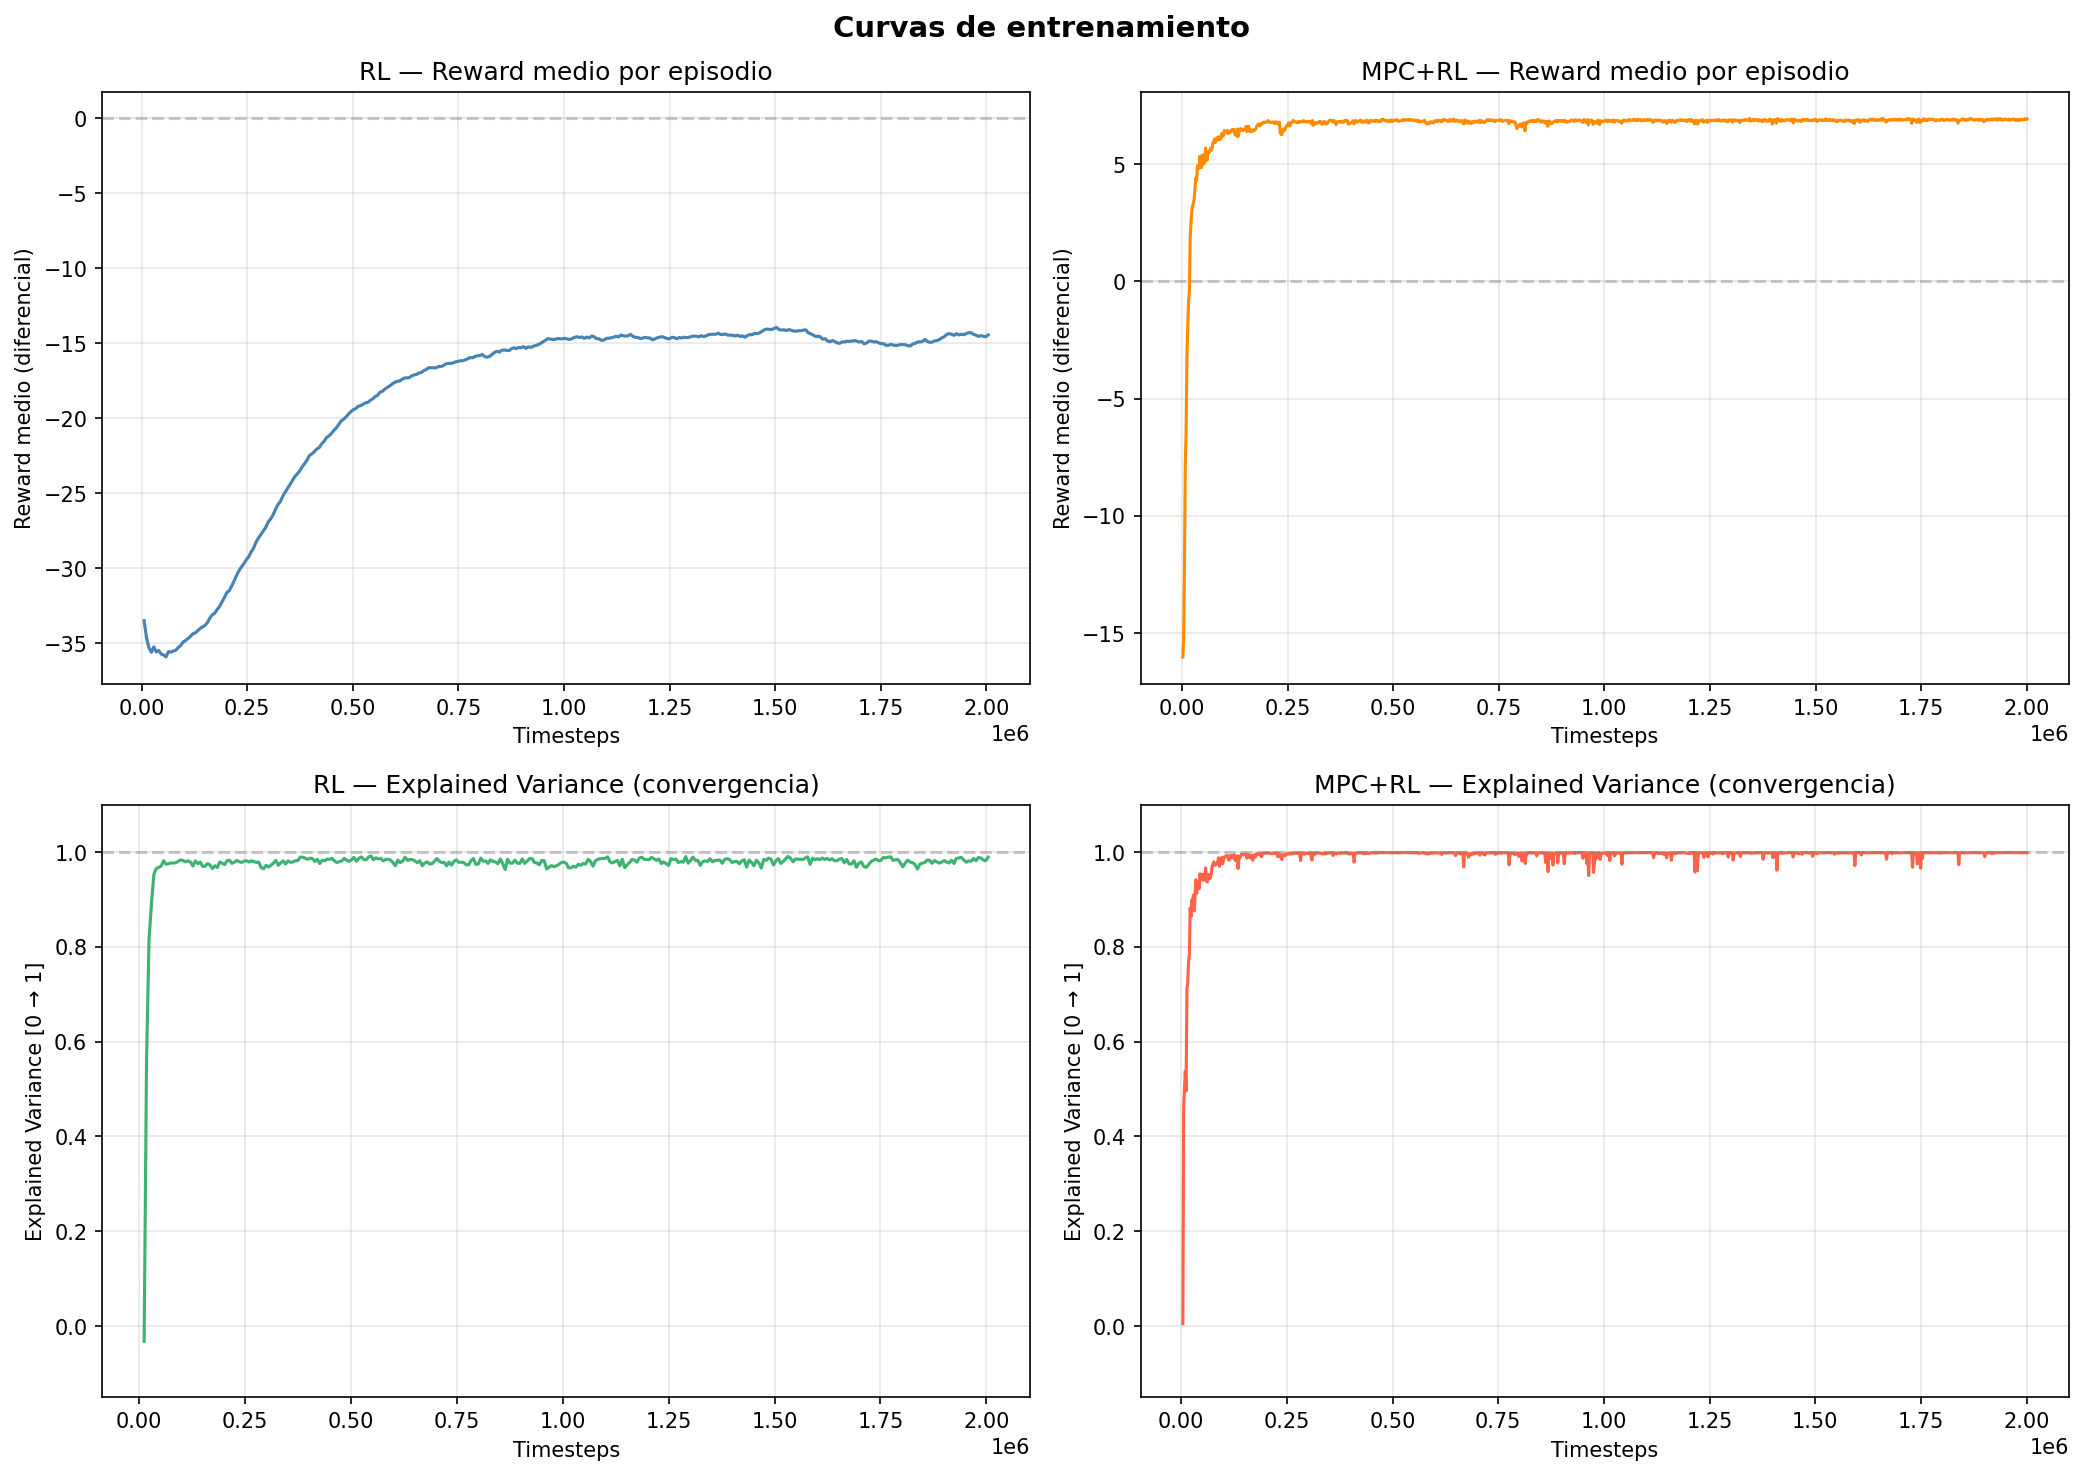
\includegraphics[width=0.95\textwidth]{imatges/training_curves.png}
\caption{Corbes d'aprenentatge de l'agent PPO i del controlador MPC+RL durant l'entrenament. El panell superior mostra la recompensa mitjana per episodi, i el panell inferior l'\textit{explained variance} del crític, utilitzada com a indicador de convergència.}
\label{fig:training}
\end{figure}

Les corbes mostren la recompensa mitjana per episodi (\textit{rolling mean} calculada per Stable-Baselines3 sobre els darrers episodis) en funció del nombre de timesteps d'entrenament. Es considera que hi ha convergència quan la recompensa s'estabilitza i l'\textit{explained variance} s'aproxima a 1, la qual cosa indica que el crític prediu correctament els retorns.

Per quantificar la variabilitat del procés d'aprenentatge i verificar la convergència de l'agent, s'ha repetit l'entrenament de l'agent PPO cinc vegades amb llavors aleatòries independents (seeds $\{0, 1, 2, 3, 4\}$), mantenint idèntics els hiperparàmetres. La Figura~\ref{fig:learning_evolution} mostra la recompensa mitjana per episodi (mitjana sobre les 5 runs) i la banda d'incertesa local del 95\,\%, calculada a partir de la desviació estàndard de la recompensa dins d'una finestra mòbil al voltant de cada punt. Aquesta banda mesura com d'estable és la recompensa en cada moment de l'entrenament: una banda ampla indica alta variabilitat local (exploració intensa) i una banda estreta indica que la \textit{policy} s'ha estabilitzat (convergència).

\begin{figure}[htb]
\centering
\begin{tikzpicture}
\begin{axis}[
  width=0.92\textwidth, height=5.5cm,
  xmin=0, xmax=1440,
  ymin=-44, ymax=-14,
  xtick={0,200,400,600,800,1000,1200,1400},
  xlabel={Episodis d'entrenament (dies)},
  ylabel={Recompensa mitjana per episodi},
  grid=both, grid style={gray!25,line width=0.3pt},
  tick align=outside, tick pos=left,
  enlarge x limits=false,
  every axis plot/.append style={no marks},
  legend style={at={(0.99,0.05)},anchor=south east,font=\scriptsize,
    cells={anchor=west},fill=white,fill opacity=0.85,text opacity=1,draw=gray!50},
]
% ── Banda IC 95 % ─────────────────────────────────────────────────────────────
\addplot[name path=CIHI, draw=none] coordinates {
  (4.0,-30.3937)(27.5,-30.0458)(51.1,-29.5414)(74.6,-28.7341)(98.1,-27.3030)
  (121.6,-25.7652)(145.2,-24.2258)(168.7,-22.8049)(192.2,-21.7737)(215.7,-21.2412)
  (239.3,-21.1694)(262.8,-21.4187)(286.3,-21.8270)(309.8,-22.2460)(333.4,-22.5107)
  (356.9,-22.6142)(380.4,-22.5945)(403.9,-22.4616)(427.5,-22.3394)(451.0,-22.1696)
  (474.5,-21.9694)(498.0,-21.7732)(521.6,-21.5829)(545.1,-21.4482)(568.6,-21.3008)
  (592.1,-21.1741)(615.7,-21.0592)(639.2,-20.9233)(662.7,-20.7986)(686.2,-20.6846)
  (709.8,-20.5234)(733.3,-20.3128)(756.8,-20.1141)(780.3,-19.8965)(803.9,-19.7336)
  (827.4,-19.6197)(850.9,-19.5152)(874.4,-19.4490)(898.0,-19.3323)(921.5,-19.2777)
  (945.0,-19.2415)(968.5,-19.1901)(992.1,-19.1980)(1015.6,-19.1350)(1039.1,-19.0798)
  (1062.6,-19.0478)(1086.2,-19.0006)(1109.7,-19.0344)(1133.2,-19.0530)(1156.7,-19.0733)
  (1180.3,-19.1194)(1203.8,-19.0920)(1227.3,-19.0993)(1250.8,-19.1315)(1274.4,-19.1048)
  (1297.9,-19.1103)(1321.4,-19.1156)(1344.9,-19.0437)(1368.5,-18.9890)(1392.0,-18.9412)
};
\addplot[name path=CILO, draw=none] coordinates {
  (4.0,-40.3146)(27.5,-40.2515)(51.1,-40.5912)(74.6,-40.7854)(98.1,-40.1379)
  (121.6,-39.1936)(145.2,-38.1020)(168.7,-36.9387)(192.2,-35.7485)(215.7,-34.6167)
  (239.3,-33.4905)(262.8,-32.2720)(286.3,-31.1372)(309.8,-30.1222)(333.4,-29.2014)
  (356.9,-28.4690)(380.4,-27.9243)(403.9,-27.4688)(427.5,-27.1181)(451.0,-26.7702)
  (474.5,-26.4025)(498.0,-26.0215)(521.6,-25.6402)(545.1,-25.3283)(568.6,-25.0275)
  (592.1,-24.7793)(615.7,-24.5598)(639.2,-24.3337)(662.7,-24.1335)(686.2,-23.9629)
  (709.8,-23.7640)(733.3,-23.5335)(756.8,-23.3198)(780.3,-23.0706)(803.9,-22.8589)
  (827.4,-22.6628)(850.9,-22.4581)(874.4,-22.2623)(898.0,-21.9998)(921.5,-21.8090)
  (945.0,-21.6235)(968.5,-21.4430)(992.1,-21.3222)(1015.6,-21.1088)(1039.1,-20.9073)
  (1062.6,-20.7114)(1086.2,-20.5115)(1109.7,-20.3997)(1133.2,-20.2705)(1156.7,-20.1693)
  (1180.3,-20.1024)(1203.8,-20.0017)(1227.3,-19.9625)(1250.8,-19.9628)(1274.4,-19.9314)
  (1297.9,-19.9300)(1321.4,-19.9406)(1344.9,-19.8831)(1368.5,-19.8379)(1392.0,-19.8010)
};
\addplot[blue!20, draw=none] fill between[of=CILO and CIHI];
% ── Línia de la mitjana ────────────────────────────────────────────────────────
\addplot[blue!70!black, line width=1.4pt] coordinates {
  (4.0,-35.3541)(27.5,-35.1487)(51.1,-35.0663)(74.6,-34.7597)(98.1,-33.7205)
  (121.6,-32.4794)(145.2,-31.1639)(168.7,-29.8718)(192.2,-28.7611)(215.7,-27.9289)
  (239.3,-27.3300)(262.8,-26.8454)(286.3,-26.4821)(309.8,-26.1841)(333.4,-25.8560)
  (356.9,-25.5416)(380.4,-25.2594)(403.9,-24.9652)(427.5,-24.7287)(451.0,-24.4699)
  (474.5,-24.1859)(498.0,-23.8974)(521.6,-23.6115)(545.1,-23.3883)(568.6,-23.1642)
  (592.1,-22.9767)(615.7,-22.8095)(639.2,-22.6285)(662.7,-22.4660)(686.2,-22.3238)
  (709.8,-22.1437)(733.3,-21.9232)(756.8,-21.7170)(780.3,-21.4835)(803.9,-21.2963)
  (827.4,-21.1412)(850.9,-20.9867)(874.4,-20.8556)(898.0,-20.6661)(921.5,-20.5433)
  (945.0,-20.4325)(968.5,-20.3165)(992.1,-20.2601)(1015.6,-20.1219)(1039.1,-19.9935)
  (1062.6,-19.8796)(1086.2,-19.7561)(1109.7,-19.7171)(1133.2,-19.6618)(1156.7,-19.6213)
  (1180.3,-19.6109)(1203.8,-19.5469)(1227.3,-19.5309)(1250.8,-19.5472)(1274.4,-19.5181)
  (1297.9,-19.5202)(1321.4,-19.5281)(1344.9,-19.4634)(1368.5,-19.4135)(1392.0,-19.3711)
};
\addlegendimage{area legend,fill=blue!20,draw=none}
\addlegendentry{IC 95\,\%}
\addlegendentry{Mitjana (5 runs)}
\end{axis}
\end{tikzpicture}
\caption{Evolució de l'aprenentatge de l'agent PPO (mitjana de 5 execucions independents, seeds $\{0\text{--}4\}$). La línia contínua és la recompensa mitjana per episodi i la banda ombrejada l'interval de confiança del 95\,\% de la variabilitat local (desviació estàndard sobre una finestra mòbil). La banda es redueix a mesura que la \textit{policy} convergeix i la recompensa s'estabilitza. Cada episodi correspon a un dia de simulació (1.440 passos d'un minut).}
\label{fig:learning_evolution}
\end{figure}

La Figura~\ref{fig:learning_evolution} confirma que la \textit{policy} convergeix de forma consistent: la banda d'incertesa local, ampla durant la fase d'exploració inicial (alta variabilitat de la recompensa), es redueix progressivament fins a estabilitzar-se en les darreres fases de l'entrenament, quan la recompensa oscil·la poc al voltant de la mitjana. Això és consistent amb el comportament esperat d'un algorisme actor-crític: primer explora i ajusta agressivament els pesos, i en les últimes iteracions fa correccions cada cop menors fins a la convergència. La convergència equivalent de l'agent MPC+RL s'il·lustra a la Figura~\ref{fig:ablacio}, on es mostren les corbes d'aprenentatge de 8 configuracions independents.

\section{Anàlisi del comportament diari}

\begin{figure}[htb]
\centering
\pgfplotsset{diatipic/.style={
  width=\textwidth, height=4.5cm,
  xmin=0, xmax=24,
  xtick={0,3,6,9,12,15,18,21,24},
  grid=both, grid style={gray!25,line width=0.3pt},
  tick align=outside, tick pos=left,
  every axis plot/.append style={no marks,line width=0.8pt},
  enlarge x limits=false,
}}
% ── Panel 1: SoC ──────────────────────────────────────────────────────────────
\begin{tikzpicture}
\begin{axis}[diatipic,
  xticklabels={,,,,,,,,},
  ylabel={SoC},
  ymin=0, ymax=1.05, ytick={0,0.25,0.5,0.75,1.0},
  legend style={at={(0.99,0.97)},anchor=north east,font=\scriptsize,
    cells={anchor=west},fill=white,fill opacity=0.85,text opacity=1,draw=gray!50},
  legend columns=2,
]
\addplot[black!40,thick] coordinates {(0,0)(24,0)};
\addplot[blue!70!black] coordinates {
  (0.000,0.0000)(0.167,0.0000)(0.333,0.0000)(0.500,0.0000)(0.667,0.0000)
  (0.833,0.0000)(1.000,0.0000)(1.167,0.0000)(1.333,0.0000)(1.500,0.0000)
  (1.667,0.0000)(1.833,0.0000)(2.000,0.0000)(2.167,0.0000)(2.333,0.0000)
  (2.500,0.0000)(2.667,0.0000)(2.833,0.0000)(3.000,0.0000)(3.167,0.0000)
  (3.333,0.0000)(3.500,0.0000)(3.667,0.0000)(3.833,0.0000)(4.000,0.0000)
  (4.167,0.0000)(4.333,0.0000)(4.500,0.0000)(4.667,0.0000)(4.833,0.0000)
  (5.000,0.0000)(5.167,0.0008)(5.333,0.0018)(5.500,0.0028)(5.667,0.0035)
  (5.833,0.0042)(6.000,0.0045)(6.167,0.0013)(6.333,0.0000)(6.500,0.0000)
  (6.667,0.0000)(6.833,0.0000)(7.000,0.0000)(7.167,0.0000)(7.333,0.0000)
  (7.500,0.0024)(7.667,0.0110)(7.833,0.0234)(8.000,0.0352)(8.167,0.0354)
  (8.333,0.0367)(8.500,0.0243)(8.667,0.0034)(8.833,0.0020)(9.000,0.0027)
  (9.167,0.0006)(9.333,0.0005)(9.500,0.0024)(9.667,0.0033)(9.833,0.0052)
  (10.000,0.0051)(10.167,0.0044)(10.333,0.0034)(10.500,0.0020)(10.667,0.0023)
  (10.833,0.0012)(11.000,0.0006)(11.167,0.0014)(11.333,0.0024)(11.500,0.0034)
  (11.667,0.0037)(11.833,0.0002)(12.000,0.0000)(12.167,0.0000)(12.333,0.0000)
  (12.500,0.0000)(12.667,0.0000)(12.833,0.0000)(13.000,0.0000)(13.167,0.0000)
  (13.333,0.0000)(13.500,0.0000)(13.667,0.0000)(13.833,0.0000)(14.000,0.0019)
  (14.167,0.0111)(14.333,0.0221)(14.500,0.0444)(14.667,0.0691)(14.833,0.0748)
  (15.000,0.0686)(15.167,0.0617)(15.333,0.0546)(15.500,0.0467)(15.667,0.0416)
  (15.833,0.0420)(16.000,0.0449)(16.167,0.0377)(16.333,0.0331)(16.500,0.0307)
  (16.667,0.0246)(16.833,0.0200)(17.000,0.0198)(17.167,0.0150)(17.333,0.0142)
  (17.500,0.0139)(17.667,0.0154)(17.833,0.0197)(18.000,0.0278)(18.167,0.0237)
  (18.333,0.0206)(18.500,0.0189)(18.667,0.0184)(18.833,0.0206)(19.000,0.0277)
  (19.167,0.0236)(19.333,0.0207)(19.500,0.0188)(19.667,0.0183)(19.833,0.0183)
  (20.000,0.0180)(20.167,0.0156)(20.333,0.0129)(20.500,0.0100)(20.667,0.0069)
  (20.833,0.0034)(21.000,0.0000)(21.167,0.0000)(21.333,0.0000)(21.500,0.0000)
  (21.667,0.0000)(21.833,0.0000)(22.000,0.0000)(22.167,0.0000)(22.333,0.0000)
  (22.500,0.0000)(22.667,0.0000)(22.833,0.0000)(23.000,0.0000)(23.167,0.0000)
  (23.333,0.0000)(23.500,0.0000)(23.667,0.0000)(23.833,0.0000)
};
\addplot[orange!85!black] coordinates {
  (0.000,0.0408)(0.167,0.0408)(0.333,0.0408)(0.500,0.0459)(0.667,0.0579)
  (0.833,0.0664)(1.000,0.0821)(1.167,0.0959)(1.333,0.1078)(1.500,0.1197)
  (1.667,0.1301)(1.833,0.1420)(2.000,0.1522)(2.167,0.1624)(2.333,0.1726)
  (2.500,0.1845)(2.667,0.1912)(2.833,0.2031)(3.000,0.2150)(3.167,0.2253)
  (3.333,0.2354)(3.500,0.2474)(3.667,0.2594)(3.833,0.2712)(4.000,0.2796)
  (4.167,0.2864)(4.333,0.2966)(4.500,0.3119)(4.667,0.3297)(4.833,0.3478)
  (5.000,0.3662)(5.167,0.3838)(5.333,0.4020)(5.500,0.4207)(5.667,0.4394)
  (5.833,0.4581)(6.000,0.4747)(6.167,0.4911)(6.333,0.5114)(6.500,0.5332)
  (6.667,0.5557)(6.833,0.5788)(7.000,0.5936)(7.167,0.5936)(7.333,0.5936)
  (7.500,0.5936)(7.667,0.5936)(7.833,0.5970)(8.000,0.6022)(8.167,0.6022)
  (8.333,0.6022)(8.500,0.5811)(8.667,0.5487)(8.833,0.5469)(9.000,0.5452)
  (9.167,0.5189)(9.333,0.4941)(9.500,0.4848)(9.667,0.4793)(9.833,0.4529)
  (10.000,0.4139)(10.167,0.3752)(10.333,0.3429)(10.500,0.3050)(10.667,0.2725)
  (10.833,0.2417)(11.000,0.2120)(11.167,0.1892)(11.333,0.1793)(11.500,0.1793)
  (11.667,0.1793)(11.833,0.1571)(12.000,0.1506)(12.167,0.1506)(12.333,0.1506)
  (12.500,0.1506)(12.667,0.1506)(12.833,0.1506)(13.000,0.1506)(13.167,0.1506)
  (13.333,0.1506)(13.500,0.1506)(13.667,0.1506)(13.833,0.1506)(14.000,0.1506)
  (14.167,0.1506)(14.333,0.1506)(14.500,0.1506)(14.667,0.1506)(14.833,0.1506)
  (15.000,0.1506)(15.167,0.1506)(15.333,0.1506)(15.500,0.1506)(15.667,0.1506)
  (15.833,0.1506)(16.000,0.1506)(16.167,0.1506)(16.333,0.1506)(16.500,0.1558)
  (16.667,0.1662)(16.833,0.1730)(17.000,0.1730)(17.167,0.1730)(17.333,0.1730)
  (17.500,0.1730)(17.667,0.1747)(17.833,0.1781)(18.000,0.1798)(18.167,0.1798)
  (18.333,0.1798)(18.500,0.1798)(18.667,0.1798)(18.833,0.1798)(19.000,0.1798)
  (19.167,0.1798)(19.333,0.1798)(19.500,0.1730)(19.667,0.1610)(19.833,0.1460)
  (20.000,0.1147)(20.167,0.0820)(20.333,0.0519)(20.500,0.0280)(20.667,0.0226)
  (20.833,0.0226)(21.000,0.0226)(21.167,0.0226)(21.333,0.0226)(21.500,0.0226)
  (21.667,0.0226)(21.833,0.0226)(22.000,0.0226)(22.167,0.0226)(22.333,0.0226)
  (22.500,0.0260)(22.667,0.0260)(22.833,0.0260)(23.000,0.0280)(23.167,0.0299)
  (23.333,0.0299)(23.500,0.0299)(23.667,0.0299)(23.833,0.0299)
};
\addplot[teal!80!black] coordinates {
  (0.000,0.0042)(0.167,0.0100)(0.333,0.0100)(0.500,0.0089)(0.667,0.0064)
  (0.833,0.0034)(1.000,0.0156)(1.167,0.1691)(1.333,0.3207)(1.500,0.4695)
  (1.667,0.6151)(1.833,0.7639)(2.000,0.9076)(2.167,0.9074)(2.333,0.9067)
  (2.500,0.9054)(2.667,0.9039)(2.833,0.9021)(3.000,0.9370)(3.167,0.9323)
  (3.333,0.9274)(3.500,0.9226)(3.667,0.9177)(3.833,0.9129)(4.000,0.9420)
  (4.167,0.9374)(4.333,0.9325)(4.500,0.9275)(4.667,0.9226)(4.833,0.9178)
  (5.000,0.9345)(5.167,0.9297)(5.333,0.9249)(5.500,0.9201)(5.667,0.9152)
  (5.833,0.9105)(6.000,0.9320)(6.167,0.9285)(6.333,0.9270)(6.500,0.9275)
  (6.667,0.9299)(6.833,0.9344)(7.000,0.9392)(7.167,0.9322)(7.333,0.9280)
  (7.500,0.9252)(7.667,0.9243)(7.833,0.9254)(8.000,0.9349)(8.167,0.9472)
  (8.333,0.9551)(8.500,0.9356)(8.667,0.9071)(8.833,0.9035)(9.000,0.9143)
  (9.167,0.9068)(9.333,0.8980)(9.500,0.9022)(9.667,0.9107)(9.833,0.9066)
  (10.000,0.9020)(10.167,0.9002)(10.333,0.9045)(10.500,0.9004)(10.667,0.9000)
  (10.833,0.8964)(11.000,0.8945)(11.167,0.8839)(11.333,0.8804)(11.500,0.8926)
  (11.667,0.9085)(11.833,0.8980)(12.000,0.9108)(12.167,0.9022)(12.333,0.9003)
  (12.500,0.9021)(12.667,0.9071)(12.833,0.9144)(13.000,0.9300)(13.167,0.9169)
  (13.333,0.9150)(13.500,0.9164)(13.667,0.9201)(13.833,0.9262)(14.000,0.9395)
  (14.167,0.9428)(14.333,0.9490)(14.500,0.9570)(14.667,0.9682)(14.833,0.9606)
  (15.000,0.9404)(15.167,0.9268)(15.333,0.9091)(15.500,0.8872)(15.667,0.8636)
  (15.833,0.8465)(16.000,0.9078)(16.167,0.8968)(16.333,0.8892)(16.500,0.8848)
  (16.667,0.8715)(16.833,0.8596)(17.000,0.9017)(17.167,0.8959)(17.333,0.8937)
  (17.500,0.8916)(17.667,0.8890)(17.833,0.8854)(18.000,0.8810)(18.167,0.8763)
  (18.333,0.8714)(18.500,0.8666)(18.667,0.8619)(18.833,0.8570)(19.000,0.8459)
  (19.167,0.7805)(19.333,0.7221)(19.500,0.6690)(19.667,0.6432)(19.833,0.6385)
  (20.000,0.6245)(20.167,0.5298)(20.333,0.4381)(20.500,0.3454)(20.667,0.2445)
  (20.833,0.1329)(21.000,0.0277)(21.167,0.0230)(21.333,0.0183)(21.500,0.0137)
  (21.667,0.0089)(21.833,0.0042)(22.000,0.0043)(22.167,0.0110)(22.333,0.0105)
  (22.500,0.0093)(22.667,0.0068)(22.833,0.0036)(23.000,0.0041)(23.167,0.0095)
  (23.333,0.0092)(23.500,0.0076)(23.667,0.0057)(23.833,0.0030)
};
\legend{MPC($H$=1),MPC($H$=60),RL,MPC+RL}
\end{axis}
\end{tikzpicture}%
\vspace{1pt}
% ── Panel 2: Potència bateria ──────────────────────────────────────────────────
\begin{tikzpicture}
\begin{axis}[diatipic,
  xticklabels={,,,,,,,,},
  ylabel={Potència bat.\ (kW)},
  ymin=-55, ymax=55, ytick={-50,-25,0,25,50},
  legend style={at={(0.99,0.97)},anchor=north east,font=\scriptsize,
    cells={anchor=west},fill=white,fill opacity=0.85,text opacity=1,draw=gray!50},
  legend columns=2,
]
\addplot[black!40,thick] coordinates {(0,0)(24,0)};
\addplot[blue!70!black] coordinates {
  (0.000,0.0000)(0.167,0.0000)(0.333,0.0000)(0.500,-0.0000)(0.667,0.0000)
  (0.833,-0.0000)(1.000,-0.0000)(1.167,0.0000)(1.333,-0.0000)(1.500,-0.0000)
  (1.667,0.0000)(1.833,0.0000)(2.000,0.0000)(2.167,-0.0000)(2.333,0.0000)
  (2.500,-0.0000)(2.667,0.0000)(2.833,0.0000)(3.000,0.0000)(3.167,0.0000)
  (3.333,0.0000)(3.500,0.0000)(3.667,0.0000)(3.833,0.0000)(4.000,-0.0000)
  (4.167,0.0000)(4.333,0.0000)(4.500,0.0000)(4.667,0.0000)(4.833,0.0000)
  (5.000,-0.0000)(5.167,0.2807)(5.333,0.3001)(5.500,0.2496)(5.667,0.2142)
  (5.833,0.2095)(6.000,-1.1893)(6.167,-0.7863)(6.333,-0.0479)(6.500,-0.0000)
  (6.667,0.0000)(6.833,0.0000)(7.000,0.0000)(7.167,0.0000)(7.333,0.0000)
  (7.500,1.8961)(7.667,3.1789)(7.833,3.8245)(8.000,-0.0000)(8.167,0.2712)
  (8.333,0.1337)(8.500,-5.9877)(8.667,-4.3882)(8.833,0.1939)(9.000,0.0029)
  (9.167,-1.1042)(9.333,0.2641)(9.500,0.4865)(9.667,0.4966)(9.833,0.0169)
  (10.000,-0.1971)(10.167,0.1920)(10.333,-1.9810)(10.500,0.1230)
  (10.667,0.1093)(10.833,-0.4257)(11.000,1.8550)(11.167,0.2814)(11.333,0.2704)
  (11.500,0.3046)(11.667,0.0386)(11.833,-1.0211)(12.000,0.0000)(12.167,0.0000)
  (12.333,0.0000)(12.500,0.0000)(12.667,-0.0000)(12.833,-0.0000)
  (13.000,0.0000)(13.167,0.0000)(13.333,0.0000)(13.500,0.0000)(13.667,-0.0000)
  (13.833,0.0000)(14.000,5.7016)(14.167,2.5421)(14.333,5.2848)(14.500,7.5484)
  (14.667,7.1396)(14.833,-1.6653)(15.000,-1.9896)(15.167,-2.1542)
  (15.333,-2.1654)(15.500,-2.2933)(15.667,-0.7030)(15.833,0.6008)
  (16.000,-2.1357)(16.167,-2.5821)(16.333,0.4990)(16.500,-1.5342)
  (16.667,-1.6879)(16.833,-1.1576)(17.000,-2.2226)(17.167,-0.7457)
  (17.333,-0.1376)(17.500,0.0449)(17.667,0.8124)(17.833,1.6645)
  (18.000,-1.3316)(18.167,-1.0238)(18.333,-0.7728)(18.500,-0.3729)
  (18.667,0.1087)(18.833,1.2260)(19.000,-1.4805)(19.167,-1.0671)
  (19.333,-0.7098)(19.500,-0.3929)(19.667,-0.0000)(19.833,0.0000)
  (20.000,-0.6674)(20.167,-0.7004)(20.333,-0.8212)(20.500,-0.9594)
  (20.667,-1.0610)(20.833,-1.0949)(21.000,0.0000)(21.167,0.0000)
  (21.333,0.0000)(21.500,-0.0000)(21.667,-0.0000)(21.833,0.0000)
  (22.000,0.0000)(22.167,0.0000)(22.333,0.0000)(22.500,-0.0000)
  (22.667,-0.0000)(22.833,-0.0000)(23.000,0.0000)(23.167,0.0000)
  (23.333,-0.0000)(23.500,0.0000)(23.667,0.0000)(23.833,-0.0000)
};
\addlegendentry{MPC (H=1)}
\addplot[orange!85!black] coordinates {
  (0.000,0.0000)(0.167,0.0000)(0.333,0.0000)(0.500,0.0000)(0.667,5.2123)
  (0.833,0.0000)(1.000,5.4706)(1.167,0.0000)(1.333,0.0000)(1.500,0.0000)
  (1.667,0.0000)(1.833,0.0000)(2.000,5.0763)(2.167,5.1552)(2.333,0.0000)
  (2.500,5.0010)(2.667,0.0000)(2.833,5.0324)(3.000,5.0782)(3.167,5.1918)
  (3.333,0.0000)(3.500,0.0000)(3.667,5.1543)(3.833,5.0260)(4.000,0.0000)
  (4.167,5.1567)(4.333,0.0000)(4.500,5.1788)(4.667,5.4519)(4.833,5.4935)
  (5.000,5.0607)(5.167,5.3752)(5.333,5.5637)(5.500,5.6105)(5.667,5.6540)
  (5.833,5.5915)(6.000,0.0000)(6.167,5.7532)(6.333,6.3722)(6.500,6.6824)
  (6.667,6.8462)(6.833,7.2302)(7.000,0.0000)(7.167,0.0000)(7.333,0.0000)
  (7.500,0.0000)(7.667,0.0000)(7.833,5.1030)(8.000,0.0000)(8.167,0.0000)
  (8.333,0.0000)(8.500,-9.6173)(8.667,-7.2582)(8.833,0.0000)(9.000,-5.0192)
  (9.167,-9.1429)(9.333,-5.8616)(9.500,0.0000)(9.667,-5.8462)(9.833,-11.9080)
  (10.000,-12.0846)(10.167,-9.4513)(10.333,-13.6308)(10.500,-9.8878)
  (10.667,-9.6499)(10.833,-10.0584)(11.000,-5.5944)(11.167,-6.5169)
  (11.333,0.0000)(11.500,0.0000)(11.667,0.0000)(11.833,-7.7288)(12.000,0.0000)
  (12.167,0.0000)(12.333,0.0000)(12.500,0.0000)(12.667,0.0000)(12.833,0.0000)
  (13.000,0.0000)(13.167,0.0000)(13.333,0.0000)(13.500,0.0000)(13.667,0.0000)
  (13.833,0.0000)(14.000,0.0000)(14.167,0.0000)(14.333,0.0000)(14.500,0.0000)
  (14.667,0.0000)(14.833,0.0000)(15.000,0.0000)(15.167,0.0000)(15.333,0.0000)
  (15.500,0.0000)(15.667,0.0000)(15.833,0.0000)(16.000,0.0000)(16.167,0.0000)
  (16.333,0.0000)(16.500,5.1416)(16.667,0.0000)(16.833,5.0529)(17.000,0.0000)
  (17.167,0.0000)(17.333,0.0000)(17.500,0.0000)(17.667,0.0000)(17.833,5.0332)
  (18.000,0.0000)(18.167,0.0000)(18.333,0.0000)(18.500,0.0000)(18.667,0.0000)
  (18.833,0.0000)(19.000,0.0000)(19.167,0.0000)(19.333,0.0000)(19.500,-5.0145)
  (19.667,-5.1291)(19.833,-7.2506)(20.000,-9.9726)(20.167,-9.1629)
  (20.333,-8.6546)(20.500,-5.8567)(20.667,0.0000)(20.833,0.0000)
  (21.000,0.0000)(21.167,0.0000)(21.333,0.0000)(21.500,0.0000)(21.667,0.0000)
  (21.833,0.0000)(22.000,0.0000)(22.167,0.0000)(22.333,0.0000)(22.500,0.0000)
  (22.667,0.0000)(22.833,0.0000)(23.000,6.1101)(23.167,0.0000)(23.333,0.0000)
  (23.500,0.0000)(23.667,0.0000)(23.833,0.0000)
};
\addlegendentry{MPC (H=60)}
\addplot[teal!80!black] coordinates {
  (0.000,12.4891)(0.167,0.2946)(0.333,-0.2328)(0.500,-0.4422)(0.667,-0.9841)
  (0.833,-0.9352)(1.000,46.7052)(1.167,45.8020)(1.333,45.1789)(1.500,44.1099)
  (1.667,43.8545)(1.833,45.2032)(2.000,-0.0102)(2.167,-0.1461)(2.333,-0.3436)
  (2.500,-0.4653)(2.667,-0.3933)(2.833,-0.5004)(3.000,-1.5300)(3.167,-1.5100)
  (3.333,-1.3200)(3.500,-1.4200)(3.667,-1.5200)(3.833,-1.5400)(4.000,-1.4400)
  (4.167,-1.4800)(4.333,-1.4200)(4.500,-1.5300)(4.667,-1.3300)(4.833,-1.3800)
  (5.000,-1.5300)(5.167,-1.4400)(5.333,-1.3700)(5.500,-1.4800)(5.667,-1.3700)
  (5.833,-1.4300)(6.000,-1.3500)(6.167,-0.9000)(6.333,-0.0700)(6.500,0.4200)
  (6.667,1.1200)(6.833,1.5100)(7.000,-2.8177)(7.167,-1.5483)(7.333,-1.1561)
  (7.500,-0.4751)(7.667,-0.1515)(7.833,0.7370)(8.000,3.6378)(8.167,3.6744)
  (8.333,-1.7997)(8.500,-8.2274)(8.667,-6.6733)(8.833,3.0549)(9.000,1.1534)
  (9.167,-4.1648)(9.333,-0.8747)(9.500,3.4665)(9.667,1.7770)(9.833,-4.0392)
  (10.000,-0.6097)(10.167,1.3417)(10.333,-2.8260)(10.500,-0.0450)
  (10.667,-0.1298)(10.833,-2.0759)(11.000,-0.1489)(11.167,-3.3479)
  (11.333,2.7496)(11.500,2.9589)(11.667,6.3659)(11.833,-5.4979)
  (12.000,-5.0608)(12.167,-1.2783)(12.333,0.0564)(12.500,1.0033)
  (12.667,1.7000)(12.833,2.7169)(13.000,-8.4372)(13.167,-1.7082)
  (13.333,0.0498)(13.500,0.6397)(13.667,1.5551)(13.833,2.1819)(14.000,0.0163)
  (14.167,1.7555)(14.333,2.1112)(14.500,2.7012)(14.667,3.8315)(14.833,-6.9100)
  (15.000,-3.4227)(15.167,-4.6064)(15.333,-5.8347)(15.500,-7.0156)
  (15.667,-6.3878)(15.833,-4.0368)(16.000,-2.7831)(16.167,-3.9218)
  (16.333,0.4990)(16.500,-2.8441)(16.667,-3.9467)(16.833,-3.2987)
  (17.000,-2.2708)(17.167,-1.2628)(17.333,-0.5500)(17.500,-0.6100)
  (17.667,-1.0100)(17.833,-1.1400)(18.000,-1.3600)(18.167,-1.3500)
  (18.333,-1.5100)(18.500,-1.4100)(18.667,-1.5100)(18.833,-1.5600)
  (19.000,-20.6165)(19.167,-18.5588)(19.333,-16.6934)(19.500,-15.2411)
  (19.667,-1.3800)(19.833,-1.4400)(20.000,-29.1080)(20.167,-27.8043)
  (20.333,-27.3509)(20.500,-28.6576)(20.667,-31.7045)(20.833,-34.2946)
  (21.000,-1.4659)(21.167,-1.2885)(21.333,-1.2978)(21.500,-1.5084)
  (21.667,-1.4618)(21.833,-1.3541)(22.000,12.8373)(22.167,0.3744)
  (22.333,-0.4183)(22.500,-0.4176)(22.667,-0.9710)(22.833,-0.9537)
  (23.000,12.3815)(23.167,0.2255)(23.333,-0.2982)(23.500,-0.5341)
  (23.667,-0.7821)(23.833,-0.8530)
};
\addlegendentry{RL}
\addlegendentry{MPC+RL}
\draw[gray,densely dashed,thin] (axis cs:0,0) -- (axis cs:24,0);
\end{axis}
\end{tikzpicture}%
\vspace{1pt}
% ── Panel 3: Context (dual y-axis) ────────────────────────────────────────────
\begin{tikzpicture}
\begin{axis}[diatipic,
  xlabel={Hora del dia (h)},
  ylabel={Generació / Demanda (kW)},
  ymin=0, ymax=65, ytick={0,15,30,45,60},
  axis y line*=left, axis x line*=bottom,
  legend style={at={(0.5,0.99)},anchor=north,font=\scriptsize,
    cells={anchor=west},fill=white,fill opacity=0.85,text opacity=1,draw=gray!50},
  legend columns=-1,
]
\addplot[green!60!black,thick] coordinates {
  (0.000,0.0000)(0.167,0.0000)(0.333,0.0000)(0.500,0.0000)(0.667,0.0000)
  (0.833,0.0000)(1.000,0.0000)(1.167,0.0000)(1.333,0.0000)(1.500,0.0000)
  (1.667,0.0000)(1.833,0.0000)(2.000,0.0000)(2.167,0.0000)(2.333,0.0000)
  (2.500,0.0000)(2.667,0.0000)(2.833,0.0000)(3.000,0.0000)(3.167,0.0000)
  (3.333,0.0000)(3.500,0.0000)(3.667,0.0000)(3.833,0.0000)(4.000,0.0000)
  (4.167,0.0000)(4.333,0.0000)(4.500,0.0000)(4.667,0.0000)(4.833,0.0000)
  (5.000,0.0000)(5.167,0.0000)(5.333,0.0000)(5.500,0.0000)(5.667,0.0000)
  (5.833,0.0000)(6.000,0.0600)(6.167,0.6500)(6.333,1.2500)(6.500,1.8500)
  (6.667,2.4400)(6.833,3.0400)(7.000,3.6200)(7.167,4.1600)(7.333,4.7000)
  (7.500,5.2300)(7.667,5.7700)(7.833,6.3100)(8.000,6.8300)(8.167,7.2500)
  (8.333,7.6800)(8.500,8.1000)(8.667,8.5200)(8.833,8.9500)(9.000,9.3600)
  (9.167,9.6600)(9.333,9.9600)(9.500,10.2600)(9.667,10.5600)(9.833,10.8600)
  (10.000,11.1500)(10.167,11.3200)(10.333,11.4800)(10.500,11.6500)
  (10.667,11.8200)(10.833,11.9900)(11.000,12.1500)(11.167,12.2200)
  (11.333,12.3000)(11.500,12.3700)(11.667,12.4400)(11.833,12.5100)
  (12.000,12.5600)(12.167,12.4300)(12.333,12.3100)(12.500,12.1800)
  (12.667,12.0500)(12.833,11.9300)(13.000,11.7900)(13.167,11.5300)
  (13.333,11.2800)(13.500,11.0300)(13.667,10.7700)(13.833,10.5200)
  (14.000,10.2500)(14.167,9.8800)(14.333,9.5100)(14.500,9.1300)(14.667,8.7600)
  (14.833,8.3900)(15.000,8.0000)(15.167,7.4700)(15.333,6.9500)(15.500,6.4200)
  (15.667,5.9000)(15.833,5.3700)(16.000,4.8400)(16.167,4.2900)(16.333,3.7300)
  (16.500,3.1800)(16.667,2.6200)(16.833,2.0700)(17.000,1.5400)(17.167,1.2900)
  (17.333,1.0300)(17.500,0.7700)(17.667,0.5100)(17.833,0.2600)(18.000,0.0000)
  (18.167,0.0000)(18.333,0.0000)(18.500,0.0000)(18.667,0.0000)(18.833,0.0000)
  (19.000,0.0000)(19.167,0.0000)(19.333,0.0000)(19.500,0.0000)(19.667,0.0000)
  (19.833,0.0000)(20.000,0.0000)(20.167,0.0000)(20.333,0.0000)(20.500,0.0000)
  (20.667,0.0000)(20.833,0.0000)(21.000,0.0000)(21.167,0.0000)(21.333,0.0000)
  (21.500,0.0000)(21.667,0.0000)(21.833,0.0000)(22.000,0.0000)(22.167,0.0000)
  (22.333,0.0000)(22.500,0.0000)(22.667,0.0000)(22.833,0.0000)(23.000,0.0000)
  (23.167,0.0000)(23.333,0.0000)(23.500,0.0000)(23.667,0.0000)(23.833,0.0000)
};
\addlegendentry{Generació solar (kW)}
\addplot[darkgray,thick,densely dashed] coordinates {
  (0.000,11.9400)(0.167,12.1000)(0.333,12.0900)(0.500,11.8900)(0.667,11.9200)
  (0.833,11.5000)(1.000,12.0500)(1.167,11.9400)(1.333,11.8700)(1.500,11.8900)
  (1.667,11.6800)(1.833,11.9400)(2.000,12.0100)(2.167,12.1200)(2.333,11.9100)
  (2.500,12.2800)(2.667,11.9000)(2.833,11.9200)(3.000,12.1200)(3.167,12.0900)
  (3.333,11.5200)(3.500,11.9800)(3.667,12.0300)(3.833,11.8200)(4.000,11.7100)
  (4.167,11.7900)(4.333,11.8200)(4.500,11.8100)(4.667,11.9700)(4.833,11.8200)
  (5.000,12.0500)(5.167,11.8500)(5.333,11.7500)(5.500,12.0800)(5.667,11.9500)
  (5.833,12.1200)(6.000,12.2300)(6.167,12.3100)(6.333,11.8600)(6.500,12.2200)
  (6.667,12.0400)(6.833,18.4800)(7.000,27.8000)(7.167,41.3400)(7.333,41.8900)
  (7.500,33.0300)(7.667,26.3600)(7.833,18.6700)(8.000,15.5100)(8.167,13.4500)
  (8.333,18.7856)(8.500,25.8177)(8.667,24.3182)(8.833,14.8140)(9.000,17.5774)
  (9.167,22.3642)(9.333,18.8280)(9.500,14.3960)(9.667,16.0500)(9.833,22.4831)
  (10.000,22.7371)(10.167,20.7426)(10.333,25.0810)(10.500,22.3300)
  (10.667,22.1700)(10.833,23.9057)(11.000,20.7138)(11.167,23.0450)
  (11.333,16.5375)(11.500,16.4366)(11.667,12.9517)(11.833,24.8211)
  (12.000,12.9300)(12.167,13.1294)(12.333,13.0181)(12.500,13.1568)
  (12.667,13.1556)(12.833,13.1843)(13.000,12.8930)(13.167,12.8518)
  (13.333,13.2205)(13.500,13.2792)(13.667,12.9580)(13.833,13.5767)
  (14.000,14.8154)(14.167,18.9442)(14.333,18.7629)(14.500,18.8716)
  (14.667,18.6404)(14.833,26.9037)(15.000,26.6429)(15.167,26.1820)
  (15.333,26.7512)(15.500,28.0104)(15.667,25.9646)(15.833,21.7489)
  (16.000,19.0131)(16.167,19.6818)(16.333,14.6510)(16.500,17.6741)
  (16.667,18.1567)(16.833,16.6387)(17.000,15.3808)(17.167,14.0628)
  (17.333,13.0900)(17.500,12.9500)(17.667,13.2400)(17.833,12.8000)
  (18.000,12.9200)(18.167,12.7900)(18.333,13.0400)(18.500,12.8800)
  (18.667,13.0600)(18.833,13.2200)(19.000,12.9100)(19.167,13.0800)
  (19.333,12.9200)(19.500,13.1300)(19.667,13.1700)(19.833,16.8600)
  (20.000,26.1800)(20.167,37.8000)(20.333,51.1100)(20.500,53.1900)
  (20.667,51.9000)(20.833,51.5700)(21.000,49.4000)(21.167,45.5900)
  (21.333,42.7300)(21.500,43.0900)(21.667,43.1500)(21.833,42.8400)
  (22.000,45.7700)(22.167,40.3200)(22.333,37.0600)(22.500,29.3300)
  (22.667,25.6500)(22.833,24.1700)(23.000,24.3400)(23.167,16.2400)
  (23.333,15.1500)(23.500,13.8000)(23.667,12.0700)(23.833,11.9100)
};
\addlegendentry{Demanda total (kW)}
\end{axis}

\end{tikzpicture}
\caption{Comportament d'un dia típic d'estiu (dia~93 del conjunt de test).
\emph{Dalt:} evolució del SoC de la bateria per als quatre controladors al llarg de les 24~hores. \emph{Centre:} potència de bateria (positiu\,=\,càrrega; negatiu\,=\,descàrrega). \emph{Baix:} generació fotovoltaica i demanda total de la comunitat (kW).}
\label{fig:dia_tipic}
\end{figure}

\section{Estudi d'ablació: funció d'activació i GAE-$\lambda$}
\label{sec:ablacio}

Per avaluar la robustesa de les decisions de disseny de la xarxa neuronal de l'agent MPC+RL, s'ha dut a terme un estudi d'ablació sistemàtic sobre l'entorn de macro-pas (60\,min/acció): 4 funcions d'activació (ReLU, Leaky ReLU, ELU, Tanh) $\times$ 2 valors del paràmetre GAE-$\lambda$ (0.95 i 1.00), cadascuna entrenada durant 500.000 timesteps amb els mateixos hiperparàmetres i el mateix 80\,\% d'entrenament. La recompensa representa el guany marginal respecte a l'escenari sense bateria; per tant, valors positius indiquen que la bateria aporta valor.

La Figura~\ref{fig:ablacio} mostra les corbes d'aprenentatge resultants, i la Taula~\ref{taula:ablacio} recull les recompenses finals.

\begin{figure}[htbp]
\centering
%
% ── Panel esquerra: efecte de la funció d'activació (λ=0.95) ─────────────────
%
\begin{minipage}[b]{0.495\textwidth}
\begin{tikzpicture}
\begin{axis}[
  width=\textwidth, height=5.8cm,
  title={\small Funció d'activació ($\lambda=0{,}95$)},
  xlabel={\small Timesteps}, ylabel={\small Recompensa marginal / episodi},
  xmin=0, xmax=510000,
  legend pos=south east, legend style={font=\scriptsize, fill opacity=0.8},
  grid=major, grid style={gray!25},
  scaled x ticks=false,
  xtick={0,100000,200000,300000,400000,500000},
  xticklabels={0,100k,200k,300k,400k,500k},
  tick label style={font=\tiny},
  title style={font=\small},
]
% ReLU — blau
\addplot[name path=rrU, draw=none, forget plot] coordinates {
  (1920,-3.920) (26880,4.980) (51840,4.980) (76800,5.258)
  (101760,5.594) (126720,6.399) (151680,6.822) (176640,6.757)
  (201600,6.849) (226560,6.854) (251520,6.877) (276480,6.871)
  (301440,6.363) (326400,6.558) (351360,6.545) (376320,6.661)
  (401280,6.770) (426240,6.806) (451200,6.863) (476160,6.881) (501120,6.887)};
\addplot[name path=rrL, draw=none, forget plot] coordinates {
  (1920,-18.897) (26880,2.705) (51840,4.505) (76800,4.497)
  (101760,5.116) (126720,5.931) (151680,6.537) (176640,6.594)
  (201600,6.745) (226560,6.667) (251520,6.638) (276480,6.770)
  (301440,6.129) (326400,6.312) (351360,6.423) (376320,6.542)
  (401280,6.616) (426240,6.716) (451200,6.743) (476160,6.725) (501120,6.699)};
\addplot[fill=blue!20, fill opacity=0.35, draw=none, forget plot]
  fill between[of=rrU and rrL];
\addplot[blue, thick] coordinates {
  (1920,-11.409) (26880,3.842) (51840,4.743) (76800,4.878)
  (101760,5.355) (126720,6.165) (151680,6.679) (176640,6.675)
  (201600,6.797) (226560,6.761) (251520,6.757) (276480,6.820)
  (301440,6.246) (326400,6.435) (351360,6.484) (376320,6.602)
  (401280,6.693) (426240,6.761) (451200,6.803) (476160,6.803) (501120,6.793)};
\addlegendentry{ReLU}
% Leaky ReLU — vermell
\addplot[name path=lrU, draw=none, forget plot] coordinates {
  (1920,-7.053) (26880,2.760) (51840,3.223) (76800,3.387)
  (101760,3.830) (126720,6.285) (151680,6.416) (176640,6.502)
  (201600,6.627) (226560,6.466) (251520,6.626) (276480,6.552)
  (301440,6.582) (326400,6.530) (351360,6.584) (376320,6.593)
  (401280,6.536) (426240,6.602) (451200,6.637) (476160,6.641) (501120,6.619)};
\addplot[name path=lrL, draw=none, forget plot] coordinates {
  (1920,-17.803) (26880,1.244) (51840,2.031) (76800,3.165)
  (101760,3.670) (126720,5.260) (151680,6.221) (176640,6.265)
  (201600,5.650) (226560,6.234) (251520,6.336) (276480,6.401)
  (301440,6.306) (326400,6.335) (351360,6.344) (376320,6.461)
  (401280,6.422) (426240,6.429) (451200,6.458) (476160,6.481) (501120,6.448)};
\addplot[fill=red!20, fill opacity=0.35, draw=none, forget plot]
  fill between[of=lrU and lrL];
\addplot[red, thick] coordinates {
  (1920,-12.428) (26880,2.002) (51840,2.627) (76800,3.276)
  (101760,3.750) (126720,5.773) (151680,6.319) (176640,6.384)
  (201600,6.139) (226560,6.350) (251520,6.481) (276480,6.476)
  (301440,6.444) (326400,6.432) (351360,6.464) (376320,6.527)
  (401280,6.479) (426240,6.515) (451200,6.547) (476160,6.561) (501120,6.533)};
\addlegendentry{Leaky ReLU}
% ELU — verd
\addplot[name path=eU, draw=none, forget plot] coordinates {
  (1920,-4.796) (26880,5.201) (51840,5.036) (76800,5.267)
  (101760,5.435) (126720,6.102) (151680,6.324) (176640,6.335)
  (201600,6.325) (226560,6.468) (251520,6.519) (276480,6.506)
  (301440,6.524) (326400,6.550) (351360,6.414) (376320,6.529)
  (401280,6.610) (426240,6.556) (451200,6.478) (476160,6.580) (501120,6.502)};
\addplot[name path=eL, draw=none, forget plot] coordinates {
  (1920,-20.468) (26880,3.158) (51840,4.658) (76800,4.470)
  (101760,4.785) (126720,5.382) (151680,5.690) (176640,5.730)
  (201600,5.725) (226560,6.040) (251520,6.163) (276480,6.115)
  (301440,6.136) (326400,6.248) (351360,6.245) (376320,6.343)
  (401280,6.254) (426240,6.394) (451200,6.255) (476160,6.313) (501120,6.258)};
\addplot[fill=green!20, fill opacity=0.35, draw=none, forget plot]
  fill between[of=eU and eL];
\addplot[green!60!black, thick] coordinates {
  (1920,-12.632) (26880,4.180) (51840,4.847) (76800,4.868)
  (101760,5.110) (126720,5.742) (151680,6.007) (176640,6.032)
  (201600,6.025) (226560,6.254) (251520,6.341) (276480,6.311)
  (301440,6.330) (326400,6.399) (351360,6.329) (376320,6.436)
  (401280,6.432) (426240,6.475) (451200,6.366) (476160,6.446) (501120,6.380)};
\addlegendentry{ELU}
% Tanh — taronja
\addplot[name path=tU, draw=none, forget plot] coordinates {
  (1920,-9.491) (26880,5.280) (51840,5.112) (76800,5.271)
  (101760,5.562) (126720,5.548) (151680,6.248) (176640,6.511)
  (201600,6.549) (226560,6.641) (251520,6.643) (276480,6.702)
  (301440,6.766) (326400,6.785) (351360,6.806) (376320,6.829)
  (401280,6.840) (426240,6.848) (451200,6.835) (476160,6.869) (501120,6.847)};
\addplot[name path=tL, draw=none, forget plot] coordinates {
  (1920,-19.840) (26880,0.769) (51840,4.553) (76800,4.545)
  (101760,4.371) (126720,4.885) (151680,5.772) (176640,6.283)
  (201600,6.295) (226560,6.505) (251520,6.384) (276480,6.565)
  (301440,6.672) (326400,6.638) (351360,6.707) (376320,6.701)
  (401280,6.760) (426240,6.753) (451200,6.753) (476160,6.726) (501120,6.786)};
\addplot[fill=orange!25, fill opacity=0.35, draw=none, forget plot]
  fill between[of=tU and tL];
\addplot[orange!80!black, thick] coordinates {
  (1920,-14.666) (26880,3.024) (51840,4.832) (76800,4.908)
  (101760,4.967) (126720,5.217) (151680,6.010) (176640,6.397)
  (201600,6.422) (226560,6.573) (251520,6.514) (276480,6.634)
  (301440,6.719) (326400,6.712) (351360,6.757) (376320,6.765)
  (401280,6.800) (426240,6.800) (451200,6.794) (476160,6.797) (501120,6.816)};
\addlegendentry{Tanh}
\end{axis}
\end{tikzpicture}
\end{minipage}
\hfill
%
% ── Panel dret: efecte del GAE-λ (ReLU) ──────────────────────────────────────
%
\begin{minipage}[b]{0.495\textwidth}
\begin{tikzpicture}
\begin{axis}[
  width=\textwidth, height=5.8cm,
  title={\small Paràmetre GAE-$\lambda$ (ReLU)},
  xlabel={\small Timesteps}, ylabel={\small Recompensa marginal / episodi},
  xmin=0, xmax=510000,
  legend pos=south east, legend style={font=\scriptsize, fill opacity=0.8},
  grid=major, grid style={gray!25},
  scaled x ticks=false,
  xtick={0,100000,200000,300000,400000,500000},
  xticklabels={0,100k,200k,300k,400k,500k},
  tick label style={font=\tiny},
  title style={font=\small},
]
% ReLU λ=0.95 — blau
\addplot[name path=r95U, draw=none, forget plot] coordinates {
  (1920,-3.920) (26880,4.980) (51840,4.980) (76800,5.258)
  (101760,5.594) (126720,6.399) (151680,6.822) (176640,6.757)
  (201600,6.849) (226560,6.854) (251520,6.877) (276480,6.871)
  (301440,6.363) (326400,6.558) (351360,6.545) (376320,6.661)
  (401280,6.770) (426240,6.806) (451200,6.863) (476160,6.881) (501120,6.887)};
\addplot[name path=r95L, draw=none, forget plot] coordinates {
  (1920,-18.897) (26880,2.705) (51840,4.505) (76800,4.497)
  (101760,5.116) (126720,5.931) (151680,6.537) (176640,6.594)
  (201600,6.745) (226560,6.667) (251520,6.638) (276480,6.770)
  (301440,6.129) (326400,6.312) (351360,6.423) (376320,6.542)
  (401280,6.616) (426240,6.716) (451200,6.743) (476160,6.725) (501120,6.699)};
\addplot[fill=blue!20, fill opacity=0.35, draw=none, forget plot]
  fill between[of=r95U and r95L];
\addplot[blue, thick] coordinates {
  (1920,-11.409) (26880,3.842) (51840,4.743) (76800,4.878)
  (101760,5.355) (126720,6.165) (151680,6.679) (176640,6.675)
  (201600,6.797) (226560,6.761) (251520,6.757) (276480,6.820)
  (301440,6.246) (326400,6.435) (351360,6.484) (376320,6.602)
  (401280,6.693) (426240,6.761) (451200,6.803) (476160,6.803) (501120,6.793)};
\addlegendentry{$\lambda=0{,}95$ (GAE)}
% ReLU λ=1.00 — vermell
\addplot[name path=r100U, draw=none, forget plot] coordinates {
  (1920,-9.781) (26880,5.353) (51840,4.745) (76800,5.021)
  (101760,5.488) (126720,6.046) (151680,6.142) (176640,6.419)
  (201600,6.515) (226560,6.530) (251520,6.586) (276480,6.488)
  (301440,6.614) (326400,6.620) (351360,6.609) (376320,6.539)
  (401280,6.585) (426240,6.536) (451200,6.618) (476160,6.591) (501120,6.573)};
\addplot[name path=r100L, draw=none, forget plot] coordinates {
  (1920,-24.055) (26880,-1.137) (51840,3.930) (76800,4.573)
  (101760,4.787) (126720,5.187) (151680,5.714) (176640,5.991)
  (201600,6.281) (226560,6.258) (251520,6.306) (276480,6.314)
  (301440,6.153) (326400,6.380) (351360,6.342) (376320,6.383)
  (401280,6.276) (426240,6.394) (451200,6.216) (476160,6.308) (501120,6.326)};
\addplot[fill=red!20, fill opacity=0.35, draw=none, forget plot]
  fill between[of=r100U and r100L];
\addplot[red!80!black, thick] coordinates {
  (1920,-16.918) (26880,2.108) (51840,4.338) (76800,4.797)
  (101760,5.138) (126720,5.617) (151680,5.928) (176640,6.205)
  (201600,6.398) (226560,6.394) (251520,6.446) (276480,6.401)
  (301440,6.383) (326400,6.500) (351360,6.475) (376320,6.461)
  (401280,6.430) (426240,6.465) (451200,6.417) (476160,6.449) (501120,6.449)};
\addlegendentry{$\lambda=1{,}00$ (MC)}
\end{axis}
\end{tikzpicture}
\end{minipage}
\caption{Estudi d'ablació sobre el model MPC+RL (500.000 timesteps, macro-pas 60\,min). \emph{Esquerra:} efecte de la funció d'activació amb $\lambda=0{,}95$. \emph{Dreta:} efecte del paràmetre GAE-$\lambda$ amb activació ReLU. La recompensa representa el guany marginal respecte a l'escenari sense bateria. La línia gruixuda correspon a la mitjana mòbil (finestra de 7 episodis) i les bandes ombrejades mostren l'interval de confiança del 95\,\% de la variabilitat observada durant l'entrenament.}
\label{fig:ablacio}
\end{figure}

\begin{table}[htb]
\centering
\small
\begin{tabular}{@{}llrr@{}}
\toprule
\textbf{Activació} & \textbf{GAE-$\lambda$} & \textbf{\textit{Reward} final} & \textbf{\textit{Reward} màxim} \\
\midrule
Tanh               & 0.95 & $6{,}828$ & $6{,}879$ \\
\textbf{ReLU}      & \textbf{0.95} & $\mathbf{6{,}816}$ & $\mathbf{6{,}872}$ \\
Leaky ReLU         & 1.00 & $6{,}671$ & $6{,}770$ \\
Tanh               & 1.00 & $6{,}661$ & $6{,}726$ \\
\midrule
Leaky ReLU         & 0.95 & $6{,}498$ & $6{,}611$ \\
ReLU               & 1.00 & $6{,}406$ & $6{,}596$ \\
ELU                & 1.00 & $6{,}387$ & $6{,}496$ \\
ELU                & 0.95 & $6{,}352$ & $6{,}575$ \\
\bottomrule
\end{tabular}
\caption{Resultats de l'estudi d'ablació sobre el model MPC+RL (500K timesteps, macro-pas 60\,min). La recompensa és el guany marginal respecte a l'escenari sense bateria; valors més positius indiquen millor rendiment.}
\label{taula:ablacio}
\end{table}

Les conclusions de l'estudi d'ablació sobre el model MPC+RL són:

\begin{enumerate}
    \item \textbf{Totes les configuracions convergeixen a valors similars.} El rang total entre la millor i la pitjor configuració és d'únicament 0{,}48 punts sobre una recompensa de $\approx 6{,}8$, menys d'un 7\,\% de variació relativa. Això indica que el \textit{tracker} MPC simplifica la tasca de l'agent i el fa força robust a la tria d'hiperparàmetres de la xarxa.

    \item \textbf{GAE-$\lambda$ no és el factor dominant en el model MPC+RL.} A diferència de l'entorn de pas minut, on $\lambda$ tenia un impacte de 8 punts, aquí les configuracions $\lambda=0.95$ i $\lambda=1.00$ apareixen barrejades al rànquing. Amb episodis de 24 macro-passos (24 hores), els retorns Monte Carlo purs ($\lambda=1.00$) no acumulen tanta variança com en episodis de 1440 passos.

    \item \textbf{ReLU amb $\lambda=0{,}95$ és la configuració original i pràcticament òptima.} Ocupa la segona posició, empatat estadísticament amb Tanh ($6{,}816$ vs $6{,}828$, diferència $<0{,}2\,\%$). ELU resulta la pitjor opció en aquest entorn, al contrari del que succeïa en el model de pas minut.

    \item \textbf{Validació de les decisions de disseny.} L'arquitectura MPC+RL d'aquest TFM utilitza ReLU i $\lambda=0{,}95$, configuració que obté el segon millor resultat i és estadísticament indistingible del millor. L'ablació confirma que les decisions de disseny originals eren encertades i que el sistema és robust a canvis en aquests hiperparàmetres.
\end{enumerate}

\section{Discussió}

Els resultats de la Taula~\ref{taula:resultats_principals} sobre 1.460 dies confirmen el rànquing: $\text{MPC+RL} > \text{RL} > \text{MPC(H=60)} > \text{MPC(H=1)}$.

\begin{itemize}
    \item \textbf{MPC(H=1) és completament inactiu.} Durant tots els 1.460 dies de test, el controlador greedy d'un sol pas no acciona mai la bateria (0~kWh carregats/descarregats, 100\% del temps inactiu). Atès que el preu de venda (0,080~€/kWh) és inferior al de compra (0,120~€/kWh), el benefici net immediat de qualsevol moviment de bateria sense excedent fotovoltaic és negatiu. Sense horitzó de predicció, el MPC(H=1) no pot anticipar períodes favorables i opta sistemàticament per la inacció. Constitueix la cota inferior del sistema: el cost de no tenir cap estratègia de control.

    \item \textbf{MPC(H=60) millora de forma marginal.} L'horitzó de 60 minuts permet anticipar la generació solar propera i actua el 7,6\% del temps, però el benefici net millora únicament en \textbf{324~€ (0,3\%)} respecte a MPC(H=1) al llarg de 1.460 dies (0,22~€/dia). El cost de degradació (442,55~€, 247 cicles) redueix dràsticament el guany brut en transaccions (766,86~€), deixant un benefici net addicional molt petit.

    \item \textbf{RL supera clarament el MPC(H=60).} L'agent PPO obté un benefici net de $-94.034{,}78$~€, millorant en \textbf{3.791,78~€ (3,9\%)} respecte a MPC(H=1), equivalent a \textbf{2,60~€/dia d'estalvi}. El resultat més destacat és la quasi-perfecta simetria entre energia carregada i descarregada: 44.583 vs 44.580 ~kWh (diferència de tan sols 2,4~kWh en 1.460 dies), fet que indica que l'agent ha après una \textit{policy} de ciclatge estructuralment estable. El RL manté un SoC mitjà de 0,230 i actua el 41,1\% del temps (23,7\% carregant i 17,4\% descarregant).

    \item \textbf{MPC+RL és el millor en totes les mètriques econòmiques.} L'arquitectura híbrida assoleix $-87.142{,}38$~€ de benefici net: \textbf{10.684,18~€ menys de pèrdua (10,9\%) que el MPC(H=1)}, equivalents a \textbf{7,32~€/dia d'estalvi}, i \textbf{6.892,40~€ millor que el RL en solitari} (4,72~€/dia addicionals). El \textit{tracker} MPC garanteix una simetria perfecta de la càrrega i la descàrrega (97.526,5~kWh en ambdues direccions) i un SoC mitjà de 0,705, cosa que reflecteix un ús eficient i sostingut de la capacitat de la bateria. A canvi d'un cost de degradació de 2.479,11~€ (1.950 cicles en 1.460 dies, 1,34 cicles/dia), el benefici brut de transaccions millora en 13.163,29~€.

    \item \textbf{Velocitat computacional.} El RL és el controlador més ràpid (0,132~ms/pas), seguit del MPC(H=1) (0,629~ms), MPC+RL (2,059~ms) i MPC(H=60) (3,768~ms). Tots quatre operen molt per sota de la granularitat d'1 minut, compatibles amb l'operació en temps real.
\end{itemize}


La Taula~\ref{taula:estalvi} resumeix l'estalvi net de cada controlador respecte a la inacció total, tant en termes absoluts com relatius i diaris.

\begin{table}[htb]
\centering
\resizebox{\textwidth}{!}{%
\small
\begin{tabular}{@{}lrrrr@{}}
\toprule
\textbf{Controlador} & \textbf{Benefici net (€)} & \textbf{Estalvi total (€)} & \textbf{Millora (\%)} & \textbf{Estalvi/dia (€)} \\
\midrule
MPC(H=1) — cota inf. & $-97.826{,}56$ & $0{,}00$          & $0{,}0\%$ & $0{,}00$ \\
MPC(H=60)            & $-97.502{,}25$ & $+324{,}31$       & $+0{,}3\%$ & $+0{,}22$ \\
RL (PPO)             & $-94.034{,}78$ & $+3.791{,}78$     & $+3{,}9\%$ & $+2{,}60$ \\
\textbf{MPC+RL}      & $\mathbf{-87.142{,}38}$ & $\mathbf{+10.684{,}18}$ & $\mathbf{+10{,}9\%}$ & $\mathbf{+7{,}32}$ \\
\bottomrule
\end{tabular}
}%
\caption{Estalvi net sobre el conjunt de test complet (1.460 dies) respecte al MPC(H=1).}
\label{taula:estalvi}
\end{table}

Les principals limitacions d'aquest anàlisi són: (1)~els preus utilitzats provenen dels CSVs del simulador i no d'una connexió directa amb el mercat real en línia, de manera que el valor de l'arbitratge temporal continua depenent del realisme d'aquestes sèries; (2)~el model de degradació lineal no captura efectes de profunditat de descàrrega (DoD) ni de temperatura, de manera que el cost real de degradació del MPC+RL (1,34 cicles/dia) podria ser superior al que aquí s'estima.


% ============================================================
\chapter{Conclusions i treball futur}
\label{cap:concl}
% ============================================================

\section{Resum de les contribucions}

Aquest TFM ha abordat el problema del control segur i econòmicament eficient d'un BESS de 50~kWh en una comunitat energètica formada per 20 habitatges i una instal·lació fotovoltaica compartida de 15~kW. Les contribucions principals han estat:

\begin{enumerate}
    \item El disseny i la implementació d'un \textbf{entorn de simulació RL} (\texttt{BessEnv}, Gymnasium) integrat amb el simulador de comunitat energètica de Martí Cabarrocas I Sánchez, amb model de degradació lineal i normalització d'observacions.
    \item La implementació de \textbf{quatre controladors}: MPC(H=1),  MPC(H=60), RL i l'arquitectura híbrida MPC+RL.
    \item L'ajust rigorós de la funció de recompensa i dels hiperparàmetres de PPO per evitar la \textit{policy} d'inacció i garantir l'aprenentatge d'estratègies actives.
    \item La validació que l'\textbf{arquitectura híbrida MPC+RL} és la més eficient sobre 1.460 dies de test: $-87.142$~€ de benefici net, reduint la pèrdua en 10.684~€ (10,9\%) respecte al MPC(H=1) i en 6.892~€ respecte al RL en solitari.
\end{enumerate}

\section{Avaluació crítica dels resultats}

Els resultats sobre el conjunt de test complet (1.460 dies) estableixen un rànquing clar i robust: \textbf{MPC+RL $>$ RL $>$ MPC(H=60) $>$ MPC(H=1)}. Els aspectes més rellevants són els següents:

\begin{itemize}
    \item L'arquitectura híbrida MPC+RL supera tots els controladors alternatius en benefici net, amb una millora del 10,9\% sobre la inacció total.
    \item L'agent RL supera el MPC(H=60) en 3.468~€ malgrat no tenir accés explícit a previsions de generació i demanda, demostrant la capacitat de generalització de la \textit{policy} apresa.
    \item La simetria quasi-perfecta del RL (44.583,0 vs 44.580,6~kWh en 1.460 dies) i la simetria exacta del MPC+RL indiquen \textit{policies} molt ben calibrades.
    \item Tots els controladors operen en temps real ($\ll 1$ minut per pas de decisió).
\end{itemize}

Les limitacions principals són les següents:

\begin{itemize}
    \item El MPC(H=1) és completament inactiu, la qual cosa el converteix en una cota inferior i no en una línia base competitiva. El MPC(H=60) és la referència més rellevant.
    \item Els preus provenen d'un simulador offline i no d'una interfície directa amb el mercat real en línia; per tant, els resultats depenen de la qualitat i representativitat d'aquestes sèries temporals.
    \item El model de degradació lineal és una aproximació conservadora que no captura efectes de DoD ni temperatura; el cost real de degradació del MPC+RL (1,34 cicles/dia) mereixeria un model electroquímic més detallat.
\end{itemize}

\section{Consideracions ètiques i legals}

Pel que fa a consideracions ètiques, aquest projecte no involucra dades personals ni privades: les dades de consum i generació simulades són sintètiques i no permeten la identificació de persones. La gestió d'una comunitat energètica real requeriria, però, el consentiment informat dels membres i el compliment del Reglament General de Protecció de Dades (RGPD) en cas de processar dades de consum individuals.

Des del punt de vista legal, el desplegament d'un sistema de control autònom sobre infraestructures energètiques compartides estaria subjecte a la normativa d'autoconsum (Reial Decret 244/2019) i a les condicions de connexió a la xarxa establertes per l'operador de distribució.

\section{Treball futur}

Les línies de treball futur més prometedores identificades en aquest TFM són:

\begin{itemize}
    \item \textbf{MPC amb horitzó real:} implementar un MPC amb horitzó de 24 hores i previsions de generació i demanda per disposar d'una línia base més exigent.
    \item \textbf{Millora de l'arquitectura híbrida:} ampliar el controlador actual incorporant previsions explícites, objectius multi-criteri o una penalització terminal més rica per millorar el seguiment del SoC objectiu.
    \item \textbf{Algoritmes alternatius:} explorar SAC (\textit{Soft Actor-Critic}) o TD3, que poden oferir millor exploració i estabilitat d'entrenament en espais d'acció continus.
    \item \textbf{Dades reals:} validar el sistema amb dades reals de consum i generació de la comunitat energètica de Cornellà.
    \item \textbf{Multi-agent RL:} en escenaris amb múltiples BESS distribuïts, explorar enfocaments d'aprenentatge per reforç multi-agent (MARL) per coordinar els sistemes d'emmagatzematge.
    \item \textbf{Validació en living lab (Exit, UdG):} com a primer pas cap al desplegament real, es proposa una primera prova experimental a la instal·lació del parc tecnològic Exit de la Universitat de Girona. Exit disposa d'un entorn de microxarxa real amb panells fotovoltaics, sistema d'emmagatzematge i connexió a la xarxa de distribució. Aquesta instal·lació permetria validar el controlador MPC+RL en condicions reals de generació i demanda, quantificant el \textit{sim-to-real gap} i identificant les discrepàncies entre el comportament simulat i el real que caldria corregir per al desplegament definitiu.
\end{itemize}


\backmatter

\bibliographystyle{ThesisStyleBreakable}
\bibliography{biblio}

\end{document}